\documentclass{cumcmthesis}

\usepackage[
    backend=biber,
    bibstyle=gb7714-2015,
    citestyle=gb7714-2015,
    backref=true
]{biblatex}

\usepackage{subcaption}
\usepackage{siunitx}
\usepackage{cleveref}
\usepackage{booktabs}
\usepackage{minted}
\usepackage{longtable}


\addbibresource[location=local]{reference.bib}

\title{}
\tihao{A}
\baominghao{01002019}
\schoolname{清华大学}
\membera{陈晟祺}
\memberb{周聿浩}
\memberc{陈智康}
\supervisor{}
\yearinput{2017}
\monthinput{09}
\dayinput{04}

\graphicspath{{figures/}}

\newcommand{\diff}{\mathop{}\!\mathrm{d}}
\newcommand{\var}{\mathrm{Var}}
\DeclareMathOperator*{\argmin}{arg\,min}

\begin{document}
%\maketitle
{\centering \zihao{3}\bfseries 二维CT扫描参数标定及基于滤波反投影算法的扫描图像重建 \par}

\begin{abstract}

本文通过几何分析、数理统计、信号处理、计算机辅助处理数据等方法,建立了存在测量误差情况下二维CT扫描参数标定的模型,通过模板标定了系统的扫描线间隔、旋转角度、旋转中心等参量。借助这些标定的参量, 我们完成了从扫描数据中重建物体几何形状、位置、吸收率等信息的任务。最后,我们定量分析了原有模型的缺陷,设计了新的标定模型以提高其稳定性与精确度,并对我们的工作进行了整体评价。

对于扫描线间隔的计算,利用数据中无重合的圆条带部分,可求扫描线被圆所截得的弦长。由于相邻扫描线之间间距相同,确定一条扫描线后可利用该间距得到其余扫描线的方程。后利用弦长及垂径定理可得到一个二元线性方程,其中一个变元为待求扫描线间距的平方。由于一个角度下有多条扫描线与圆相交,可以列出一组超定的方程组,后利用二元线性回归即可求得扫描线间距。由于有多个旋转角度,我们对于每个旋转角度都计算一次回归,最后对得到的数据求平均值,即得扫描线间距为$0.2766\,\si{mm}$。

旋转角度的计算与上述过程类似,利用扫描线被椭圆截得的弦长,可列出一组含其中一条截距以及斜率的非线性方程,对相邻方程进行求解可得到一组斜率值,均值作为当前角度的正切值。在旋转角接近$90^\circ$时会出现数值上的问题,此时选用斜率倒数以及$x$轴截距作为变元即可。求得系统与托盘的初始夹角为$\theta_0=29.6422^\circ$。具体的180个旋转角可见附录中表\ref{table:roration_degrees}。

在特定角度下,由线间隔可以精确地确定圆心投影位置,再加上系统旋转后圆心在旋转坐标系中坐标的变化等约束,可构造多个方程组求解旋转坐标系的原点坐标。对所有值取平均即得到旋转中心$(-9.2383, 6.2663)\si{mm}$,位于托盘中心的略左上方处。

图像的重建问题等价于逆 Radon 变换。一种算法为像素驱动的直接反投影,即计算待求像素在各个旋转角上的投影位置。其最终吸收率为其各个旋转角上投影位置上的吸收值之和。此外,可利用线性插值来将吸收值连续化。由于直接反投影带来图像模糊等问题,我们利用Fourier中心切片定理推导出了一种能较精确地还原原始信息的滤波反投影算法,即将各角度下的投影值与R-L滤波函数卷积后的值进行直接反投影。实验证明此方法是优秀的 ,恢复的图像可见附录中图\ref{fig:4_filter_copy},题中要求的10点吸收率可见附录中表\ref{table:absort_rate},详细各点吸收率可见附件。

此外,在测量值有误差的假设下,我们证明了计算出的扫描线间隔的精确度和圆模型的半径成正相关;以及旋转角度的求解结果在扫描线与椭圆的轴接近平行的临界情况下变得不稳定。为此,可利用多模板多次扫描的方法将圆与椭圆的信息解耦合,并且增大圆的半径来提高计算 扫描线间隔的精确度。对于旋转角度的不稳定性,可用椭圆在坐标系中不同的放置方式获取多组数据,最后取最小方差的角度值作为真实值。

最后,我们回顾了整个模型,分析其优点和不足之处,并对其将来的应用提出展望。

\keywords{医学影像\quad 图像重建\quad 参数标定\quad Radon变换\quad 信号处理}
\end{abstract}


\section{问题重述}
CT是医学、生物领域重要的成像手段,可以有效获取样品的 内部结构信息。题目给出了一种典型的二维CT系统,平行入射的X射线垂直于探测器平面,经过样品吸收后被等距排列的512个探测器单元接收。每次扫描过程中,整个发射-接受系统绕着旋转中心逆时针旋转180次,得到180组接收信息。

由于现实中CT系统存在误差,故需要借助已知结构的样品(模板)对系统的参数进行标定,并据此对未知结构的样品进行成像。

本题目要求建立数学模型,解决以下问题:

\begin{enumerate}
  \item 根据已知的模板几何信息和扫描结果,确定CT系统的旋转中心、探测器单元距离与180个旋转方向
  \item 根据上述标定的信息,从扫描数据中恢复出未知介质的位置、形状、吸收率
  \item 分析上述标定的精度和稳定性,设计新模板、建立标定模型以改进这些指标
\end{enumerate}

\section{问题分析}

问题1要求从已知的几何信息和扫描结果中恢复出系统的一系列参数。根据比尔-朗伯定律可知,在吸收率恒定的情况下,X射线的吸收值(即给出的测量值)与穿过物体的厚度成正比,故本小题中吸收值也可以作为物体厚度的一种度量尺寸;又由于两条X射线之间的间距恒定,故其亦可作为度量单位。再加上题目本身给出的SI制与$256\times256$两种度量,共有四种尺度。因而解决本题时尤其要注意各个尺度之间的换算和处理。我们使用每个圆中不同扫描线的长度处理得到扫描线宽,最后所有值平均得到真实线宽(即接收器间距)。由于圆直径最长,而数据中属于圆的吸收值部分出现多次明显的最大值,据此可得到圆直径在吸收值尺度下的值,也就得到了吸收值尺度与真实尺度的换算关系。对于不重叠部分,通过扫描线长处理可得到实际圆心的投影坐标。而后,在旋转中心建立另一坐标系,通过椭圆弦长与坐标系旋转的位置关系等几何约束列出方程组,可确定每一组数据对应的旋转角度(即180个方向)。再通过坐标系旋转后圆心坐标的变化等约束,可求解圆心在旋转坐标系中的坐标,也就确定了旋转中心相对托盘的位置。

问题2、3要求根据问题1中得到的参数,从扫描数据中重建介质的二维图像,即重建各点的吸收率信息,这显然是对第一题获得信息的一种检验。在求得旋转中心位置后,很容易在旋转坐标系和静止坐标系间进行变换。最简单的思路是对于每个旋转角度,将投影信息反向投影到原坐标系中;最后所有角度的信息叠加,就能得到大致的原图像。但显然这种方法的的准确度不够高,会造成各点处强度值的平均化,因此需要通过更精细的处理方法获得更接近的原始图像。

问题4要求分析问题1中参数标定的精度与稳定性,以及设计新模板、建立新模型,题目要求比较开放。这要求我们在完成问题1后,对数据的处理过程进行定量的分析。除了题中要求的接收器间距、转动角度、转动中心位置等重要物理量外,还应该对求解这些量的中间过程和理论推导进行研究。对同一个量多次估计的方差、关于同一量的超定方程组解的情况等都可以成为重要的量化指标。同样地,在设计新模板和新的标定模型时,也应当着重关注这些指标,以尽可能低的成本、尽可能简单的方式,做到精确而稳定地标定系统的各项参数。

\section{模型假设与符号约定}

在本题的求解过程中,我们做出以下基本假设:

\begin{assumption}
探测平台的180个旋转方向在每次扫描时是不变的。
\end{assumption}

\begin{assumption}
X射线在非被测介质中无损耗传播,不发生衰减、吸收。
\end{assumption}

\begin{assumption}
X射线在任何情况下中不发生散射、反射。
\end{assumption}

\begin{assumption}
所有的X射线发射器与接收器均没有损坏。
\end{assumption}

在建模与求解过程的中,我们使用了表\ref{table:symbol}中定义的一些记号。

\begin{table}[htbp]
\centering
\caption{本文中使用的记号}
\label{table:symbol}
\begin{tabular}{@{}ll@{}}
\toprule
符号          & 说明                           \\ \midrule
$s$         & 下标后缀:以接收器间隔为尺度的长度量           \\
$i$         & 下标后缀:以吸收量为尺度的长度量             \\
$\mu(x,y)$  & 介质在$(x,y)$点的衰减系数分布函数          \\
$F(u,v), F(\rho,\theta)$  & 衰减系数分布进行二维Fourier变换的结果的直角坐标与极坐标形式 \\
$g_\theta(R), \hat{g}_\theta(R)$ & 探测系统转动角度为$\theta$时位于坐标$R$处的投影的真实值与滤波值 \\
$\mathcal F_1, \mathcal F_1^{-1}$ & 一维空间中的Fourier变换与逆变换算子\\
$xoy$       & 以托盘中心为原点建立的直角坐标系             \\
$XOY$       & 以探测系统旋转中心为原点建立的坐标系           \\
$l$         & 两个相邻接收器间的距离                  \\
$R$         & 模型中小圆的半径                      \\
$a, b$      & 模型中椭圆$ox$与$oy$方向的半轴长         \\
$L_m$       & 线长:通过介质的第$m$条射线处的介质厚度        \\
$D_m$       & 线距:通过介质的第$m$条射线与最靠近第$0$条线的圆切线的距离    \\
$\theta$    & $oxy$坐标系相对于其原始状态逆时针旋转的角度     \\
$\omega, k$ & 扫描线与$oxy$坐标系$ox$正方向的夹角及其对应斜率 \\
$C(X_0,Y_0)$   & $XOY$坐标系初始状态下小圆圆心的坐标 \\ \bottomrule
\end{tabular}
\end{table} 

\section{模型建立与问题求解}

\subsection{问题1}

\subsubsection{理论支撑}

根据物理学知识可知,物体对电磁波的吸收遵循\emph{比尔-朗伯定律(Beer–Lambert law)}。其内容为:一束单色光照射于一吸收介质表面,在通过一定厚度的介质后,由于介质吸收了一部分光能,透射光的强度就要减弱。吸收介质的浓度愈大,介质的厚度愈大,则光强度的减弱愈显著。具体地,如果将X射线某条路径上的介质切分为多个厚度为$w$的微小单元,第$i$个单元的衰减系数为$\mu_i$,射线强度为$I_i$,则我们有:
\begin{equation}\label{equ:1_law}
  I_i = I_{i-1}\mathrm{e}^{-\mu_{i}w}
\end{equation}
当切分数量趋向于无穷大时,求和转化为路径积分,容易得到:
\begin{equation}\label{equ:1_integral}
    \int_{l} \mu(x, y)\diff l = \ln{\frac{I_0}{I}}
\end{equation}
其中$I$是路径末端接收到的射线强度,$I_0$是射线源强度,右侧整体称为吸收值,$\mu(x, y)$是路径上衰减系数的分布函数。

\subsubsection{数据处理与尝试}

当$\mu(x, y)$为常数时,公式\ref{equ:1_integral}左侧则为此路径上垂直于射线的介质的厚度,故在本小题的条件下(所有有介质处吸收率均为1),射线的吸收值与其经过的介质厚度成正比。我们在本小题解答过程中,将吸收值作为一个尺度度量,所有在此尺度下的长度量均以$i$作为下标结尾。同时我们也将两个接收器之间的间距作为单位长度定义一个尺度,所有在此尺度下的长度量均以$s$作为下标结尾。有特殊说明的情况除外。

\begin{figure}[htbp]
  \centering

  \begin{subfigure}[b]{0.3\textwidth}
    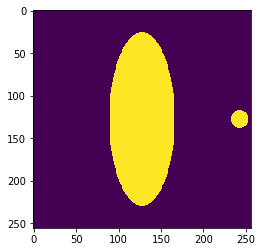
\includegraphics[width=\linewidth]{1_shape.png}
    \caption{给定介质的形状}
    \label{fig:1_data_plots:shape}
  \end{subfigure}%
  \hfill
  \begin{subfigure}[b]{0.3\textwidth}
    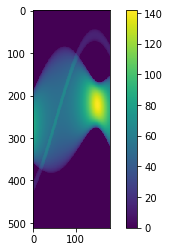
\includegraphics[width=\linewidth]{1_origin_data.png}
    \caption{原始扫描数据}
    \label{fig:1_data_plots:orig_data}
  \end{subfigure}%
  \hfill
  \begin{subfigure}[b]{0.2\textwidth}
    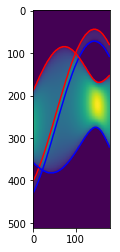
\includegraphics[width=\linewidth]{1_data_with_bounds.png}
    \caption{含边界的扫描数据}
    \label{fig:1_data_plots:orig_data_with_bounds}
  \end{subfigure}

  \caption{原始数据处理}
  \label{fig:1_data_plots} %% label for entire figure
\end{figure}

图\ref{fig:1_data_plots:shape}为题目给出的介质模板形状,我们以其中心(也是椭圆的中心)为原点建立笛卡尔坐标系$xoy$,对于此图$x$轴向右,$y$轴向上。同时我们以待求的探测系统的旋转中心为原点再建立笛卡尔坐标系$XOY$,$Y$轴正方向从接收器垂直指向探测器,$X$轴正方向指向接收器横坐标增大的方向。对于探测系统的接收器,坐标定义为:在数据第$i$行的接收器横坐标为$i - 255.5$;所有接收器纵坐标相等,规定为$-500$(只要探测器都在介质之外,其纵坐标大小不影响接受值)。

图\ref{fig:1_data_plots:orig_data}为根据题目给定的对模板的测量数据绘制的图,横轴为180个方向,纵轴为探测器编号,点颜色亮度表示吸收值。可知图中任意一条垂直线的宽度即为当前垂直X射线方向(即为平行探测器方向)的模型的宽度。图中有一条较明显的高度相同的正弦曲线形状的条带,容易推断为模板中圆形留下的图样;另一条宽度变化的条带,则为椭圆留下的图样。

首先进行较为粗略的数据提取,找到两条条带各自的边界(即,检测到吸收的接收器的范围)。方法思路为使用Python读取每一列数据,找到吸收值突变点。在两条带未重合的部分,识别十分简单。在重合部分,方法为从附近的未重合部分向上下进行试探,寻找最大值(观察可知图形上重合部分属于椭圆条带的边界比较亮)。图\ref{fig:1_data_plots:orig_data_with_bounds}为用此方法寻找到的两条带边界,基本与图形相吻合。但经过观察可知,条带图在峰、谷部分的边界并不明显(在数据上表现为各点值较接近,在图形上表现为边界线变“平”,边缘“黯淡”),这是由于接收器间具有一定的间隔造成的。故用这种方法得到的边界并不准确,无法直接用于后续计算。

\subsubsection{计算接收器间距与圆心位置}
\label{sec:1_calc_l}
\begin{figure}[htbp]
  \centering

  \begin{subfigure}[b]{0.48\textwidth}
    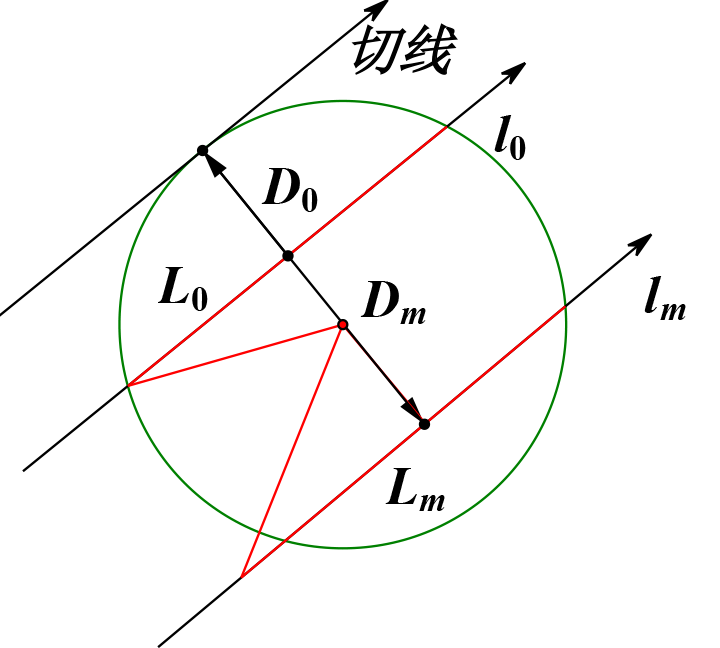
\includegraphics[width=\linewidth]{1_circle_lines.png}
    \caption{扫描线与圆的几何关系}
    \label{fig:1_circle_lines}
  \end{subfigure}%
  \hfill
  \begin{subfigure}[b]{0.48\textwidth}
    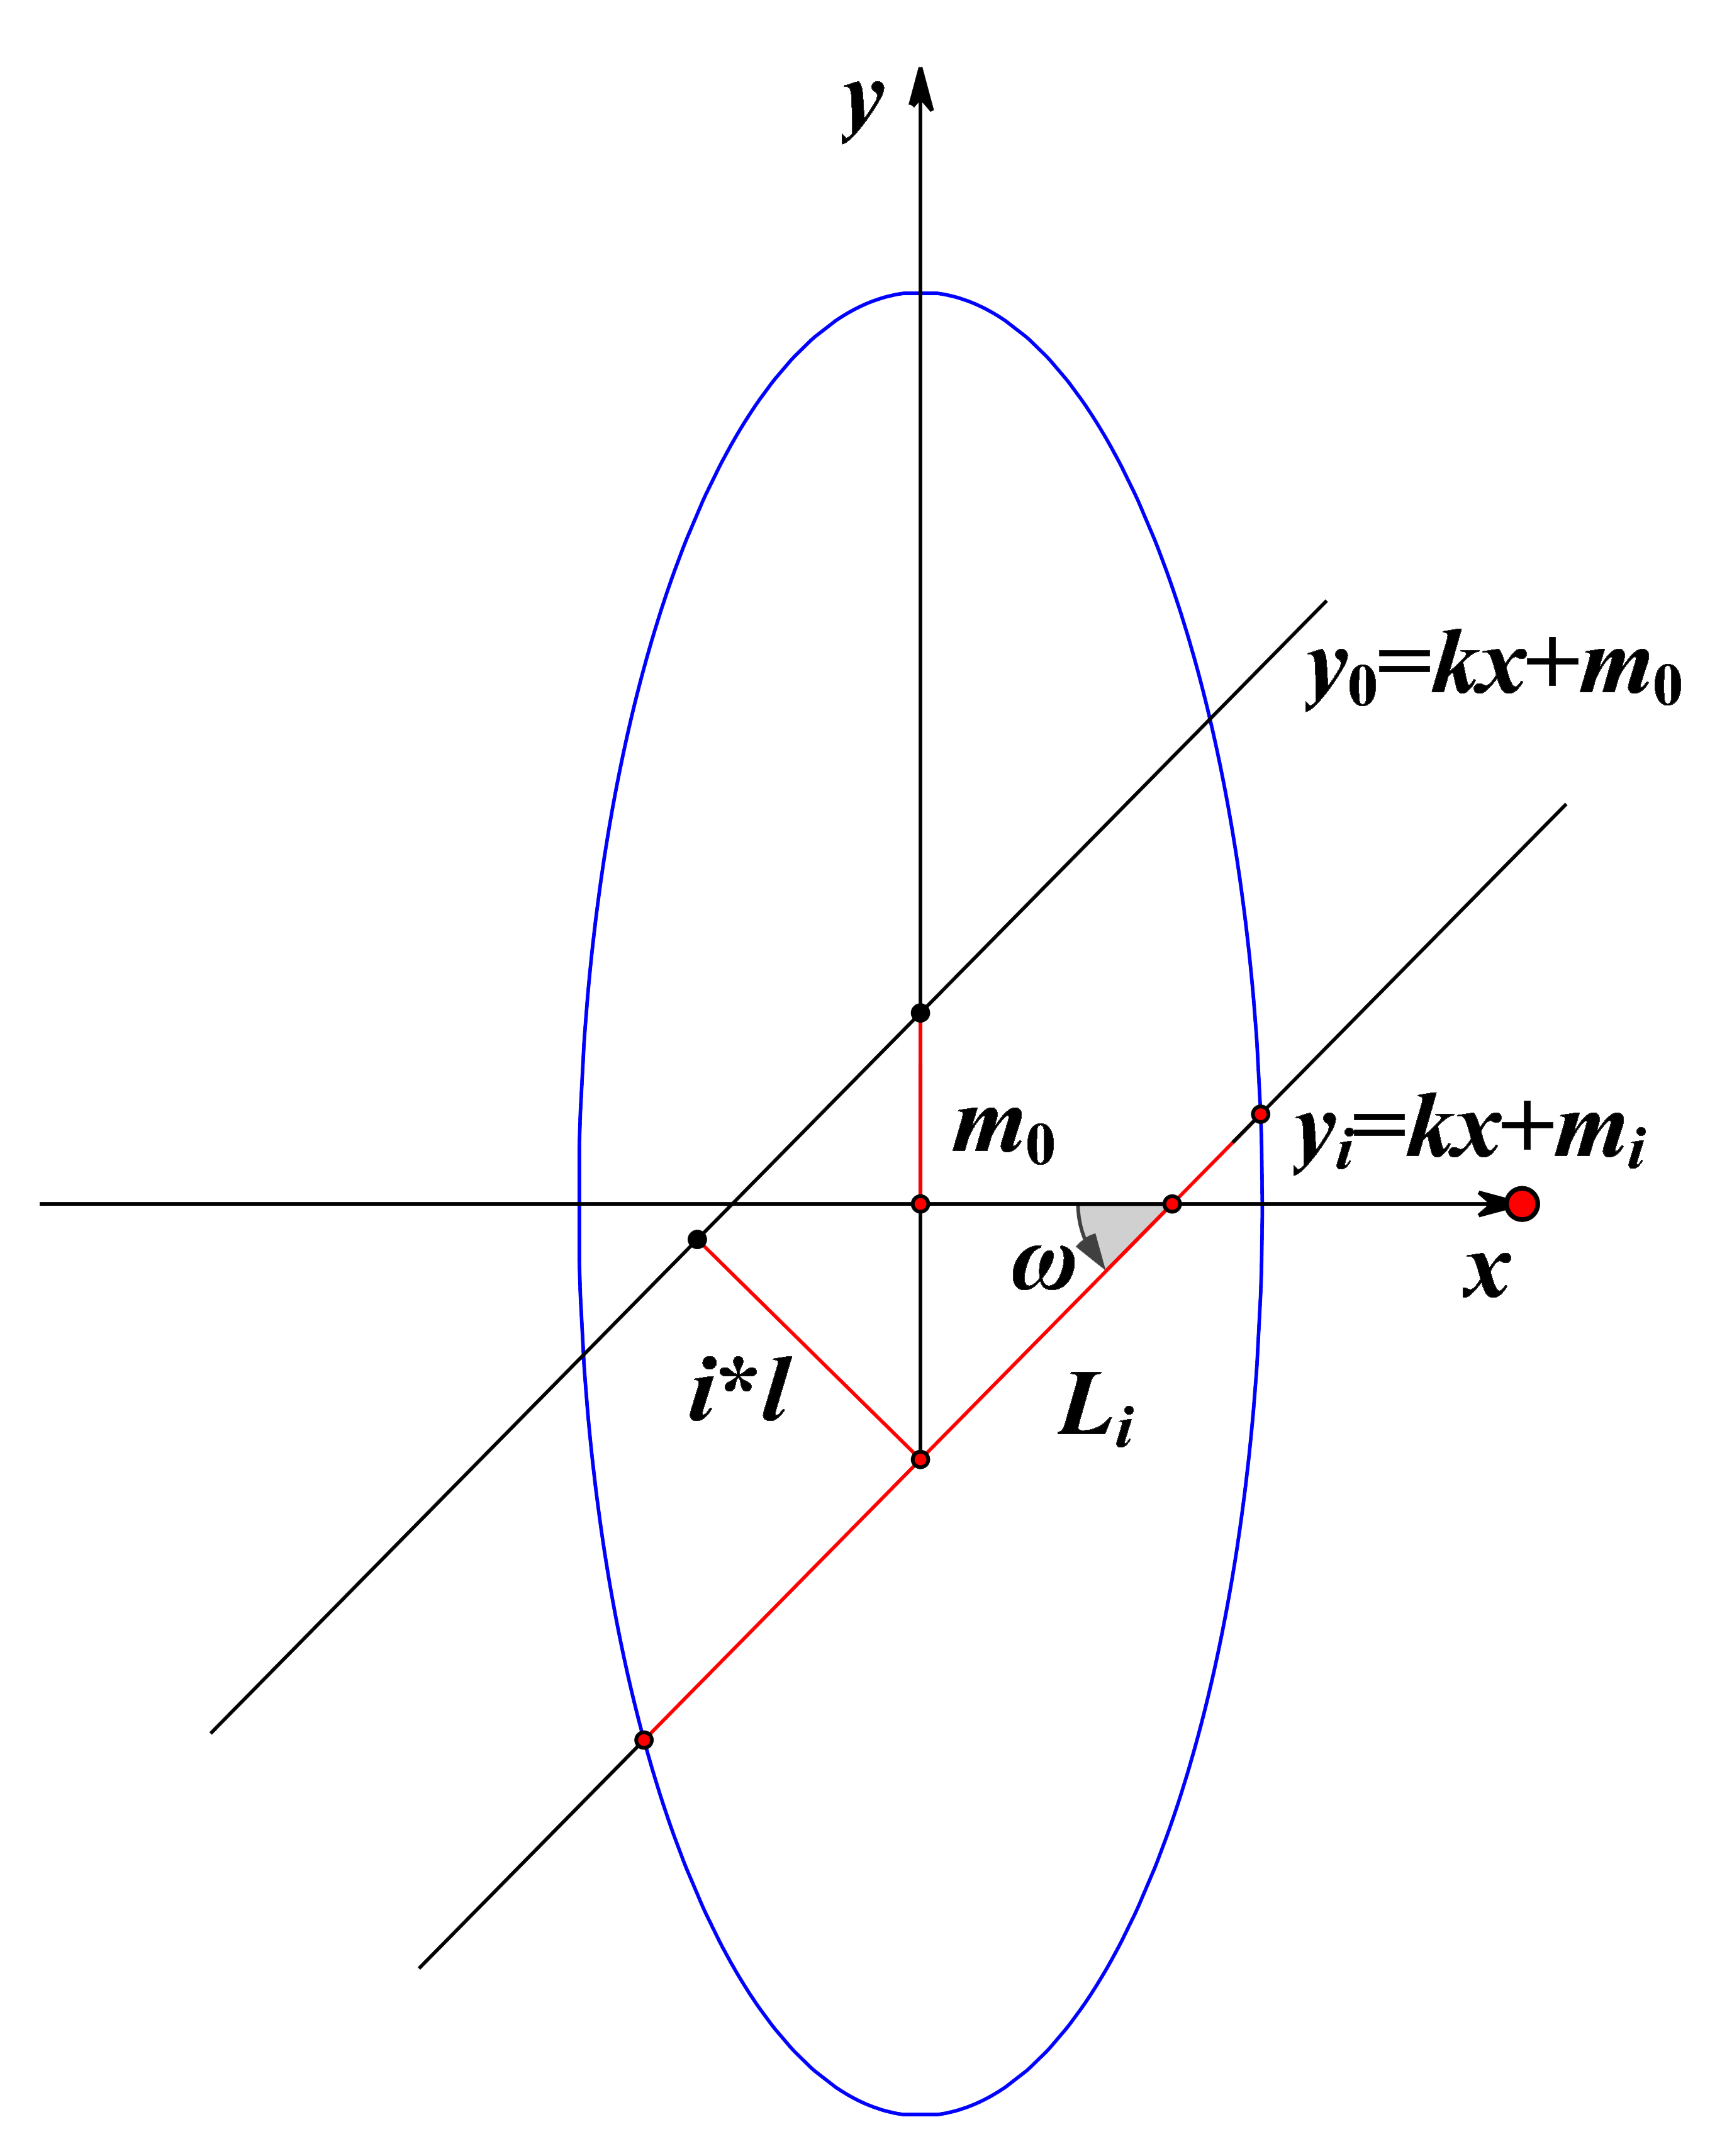
\includegraphics[width=\linewidth]{1_ellipse_lines.png}
    \caption{扫描线与椭圆的几何关系}
    \label{fig:1_ellipse_lines}
  \end{subfigure}%

  \caption{计算时几何关系的图示}
  \label{fig:1_geometry}
\end{figure}

考虑另一种思路,对于条带未重合时的数据,可精确地得知穿过圆的扫描线(即一个接收器接收到的信号)位置。下面的推导均在吸收值尺度下进行。考虑一个特定的方向,将这些线按接收器编号升序记为$l_0, l_1, \hdots, l_n$,共$n+1$条,对于第$m$条线定义“线长”即为对应接收器的读数$L_m$,定义“线距”$D_m$为第$m$条线与此方向下最靠近$l_0$的圆的切线之间的距离。根据图\ref{fig:1_circle_lines}中所描绘的几何关系,我们有
\begin{equation}\label{equ:1_circle}
  R^2=(D_m-R)^2+(\frac{L_m}{2})^2
\end{equation}
又由于$D_m=D_0+m l$,代入公式\ref{equ:1_circle}后与$m=0$时的情况相减,可得到
\begin{equation}\label{equ:1_reg}
  2 m l(D_0-R) + m^2 l^2 = \frac{L_0^2-L_m^2}{4}
\end{equation}
将$l(D_0-R)$与$l^2$作为未知系数,$2m$与$m^2$作为参数进行线性回归,可得到在这个方向下$l^2$的值。对所有条带未重合的方向重复该操作,取平均值,可得到$l_i=0.4903$(在SI制下$l=0.2766\,\si{mm}$)。这组数据的标准差为$\num{9.74e-4}$,稳定程度较高。

由于圆直径最长,而数据中属于圆的吸收值部分出现多次明显的最大值,故我们直接将每个旋转方向上吸收值最大值视为圆直径,再取这些值中的最大值后得$d_i=14.1796$。计算特定角度下圆心在旋转坐标系中的$X$坐标的方法也是简单的:在经过圆的所有扫描线中去掉线长$L_m$最大的两个$l_{max}, l_{max+1}$(一定相邻),则$l_0, l_1, \hdots, l_{max-1}$与$l_{max+2}, l_{max+3}, \hdots, l_n$分列圆心两侧,根据垂径定理(即公式\ref{equ:1_circle})即可计算出圆心与直线的距离,即可得到圆心的横坐标。对第$j$个旋转角度取得的所有坐标取均值,确定为该方向上圆心的横坐标$C_{x_j}$。当圆心横坐标确定后,我们根据横坐标与半径即可对于无重叠的部分圆条带重新确定一个更精确的边界,此边界的数值不再只落在接收器代表的点上。

\subsubsection{确定旋转角度与旋转中心}

由于探测系统所在的坐标系旋转时圆在其横轴上留下的投影位置发生变化,根据几何约束可求解旋转系统在每次投影时的旋转角度与其旋转中心相对模板的位置。具体推导如下(下列推导中,所有长度量的度量均以吸收量为尺度,略去尺度下标):

在$oxy$系中,考虑椭圆$x^2/a^2+y^2/b^2=1$(其中$a$、$b$分别为已知的两个半轴长)与扫描线$y=kx+m$,联立方程,根据解析几何知识容易知道直线截椭圆的弦长为:
\begin{equation}\label{equ:1_length}
  L = \sqrt{1+k^2}\sqrt{(x_1+x_2)^2-4 x_1 x_2} = \sqrt{k^2+1} \sqrt{\frac{4 a^4 k^2 m^2}{\left(a^2 k^2+b^2\right)^2}-\frac{4 a^2 \left(m^2-b^2\right)}{a^2 k^2+b^2}}
\end{equation}
将$XOY$系的两个轴正方向均与$oxy$系相同时的状态称为“初始位置”,当系统相对初始位置旋转角度为$\theta$时,扫描线与$ox$轴的夹角满足$\omega = \theta + \frac{\pi}{2}$。由于所有扫描线都是平行的,故第$i$条直线的截距$m_i$可以表示为$m_0+i\Delta m$,又由于$\Delta m = l / \cos(\pi-\omega) = -l/\cos\omega$,且$k=\tan\omega$。上述等式均可简单地由图\ref{fig:1_ellipse_lines}中表述的几何关系推导出。此时,方程\ref{equ:1_length}可约化为:
\begin{equation}\label{equ:1_degree_full}
  \sqrt{k^2+1} \sqrt{\frac{4 a^4 k^2 \left(i l \sqrt{k^2+1} +m_0\right){}^2}{\left(a^2 k^2+b^2\right)^2}-\frac{4 a^2 \left(\left(i l \sqrt{k^2+1} +m_0\right){}^2-b^2\right)}{a^2 k^2+b^2}}=L_i
\end{equation}

对于穿过椭圆的每一根直线,其$i$与$L_i$的值是确定的,于是方程\ref{equ:1_degree_full}便构成一个关于$k$与$m_0$的二元方程。在每一个方向上,都有足够多的扫描穿过椭圆(且不穿过圆),构成一个方程数量远多于未知数的超定方程组。我们将其相邻两两联立求解,舍去无用的$m_0$后将获得的$k$的绝对值(由于方程中均为关于$k$的偶次项,故一定会有正负两个根)进行平均,作为该方向上的扫描线斜率。在扫描线与$ox$轴接近垂直的角度上,三角函数会产生较大的误差,此时我们将直线方程重新设为$x=py+q$进行求解,求得的$|p|$为实际斜率绝对值的倒数。

在获得所有方向的$|k_i|$后,可据此计算出$\theta_i$的值;在一些临界值处的取值,是参考扫描数据的变化给出的。具体计算公式为:
\begin{equation}\label{equ:1_k_to_theta}
  \theta_i=
  \begin{cases}
    \frac{\pi}{2}-\arctan k_i, &  0 \leq i \leq 61 \\
    \frac{\pi}{2}+\arctan k_i, &  61 \leq i \leq 150 \\
    \frac{3\pi}{2}-\arctan k_i, & 151 \leq i \leq 179
  \end{cases}
\end{equation}
特别地,我们确定了第一组扫描数据对应的$\theta_0 = 0.51735\,\mathrm{rad} = 29.6420 \deg$

下一步确定旋转中心。初始位置中圆形的圆心在$XOY$系中坐标记为$C(X_0,Y_0)$,到$O$的距离$d=\sqrt{X_0^2+Y_0^2}$恒定。旋转中心在$oxy$系中的坐标即为$(-X_0,-Y_0)$。当$XOY$旋转$\theta$角度时,射线$OC$与$OX$轴形成有向角$\phi_\theta=\arg(X_0+iY_0)-\theta$(其中$i$为虚数单位),于是得到$C$的纵坐标$X_\theta=d\cos\phi_\theta$。由于在上面的过程中我们已经得到了部分旋转角度下比较精确的圆心坐标,将$\theta_i$与对应的$C_{x_i}$代入上面的推导即可获得关于$X_0$与$Y_0$的两个方程。由于数据较多,我们选取了两段未与椭圆重叠的圆条带(扫描序号分别为$0 \leq n \leq 13$与$110 \leq n \leq 180$),每次在两个集合中各选择一个扫描数据进行方程求解,共产生$910$组解。将其分别平均后得到的解为(在扫描线间距的尺度下)$X_{0\_s}= 196.0739, Y_{0\_s}= -22.6529$,转换尺度后易知探测系统的旋转中心在SI制下在$oxy$系中的坐标为$(-9.2383\,\si{mm}, 6.2663\,\si{mm})$,即位于模型板中心的略左上方位置处。

\subsection{问题2、3}
问题2与问题3的性质相同,均属于使用扫描得到的数据重建样品的吸收率分布(即形状),故二者可合并解决。

\subsubsection{数学原理:反投影}
本题要解决的问题实际为逆 Radon 变换,这个问题最早由数学家Johann Radon在1917年提出\cite{radon1986}。我们首先进行理论上的推导。

对于二维密度函数 $\mu(x, y)$,将其进行二维Fourier变换后所得的函数记为 $F(u, v)$,根据Fourier逆变换公式可以得到

\begin{equation}
	\mu(x, y) = \iint F(u, v) \mathrm e^{2\pi i(ux + vy)} \diff u \diff v
	\label{equ:2_inv_fourier}
\end{equation}

将空域变换为极坐标形式 $u = \rho\cos\theta, v = \rho\sin\theta$ 后可得

\begin{equation}
	\begin{aligned}
	\mu(x, y) &= \int_0^\infty\int_0^{2\pi} F(\rho, \theta) \mathrm e^{2\pi i \rho R} \rho\diff \theta \diff \rho \\
			&= \int_0^\infty\int_0^{\pi} F(\rho, \theta) \mathrm e^{2\pi i \rho R} \rho\diff \theta \diff \rho
			 +\int_{-\infty}^0\int_0^{\pi} F(-\rho, \theta + \pi) \mathrm e^{2\pi i \rho R} \rho\diff \theta \diff \rho
	\end{aligned}
	\label{equ:2_polar_inv_fourier}
\end{equation}

其中 $R = x\cos\theta + y\sin\theta$。由于$\mu(x, y)$为实值函数,其二维Fourier变换满足$F(\rho, \theta) = F(-\rho, \theta + \pi)$,因此

\begin{equation}
	\begin{aligned}
		\mu(x, y) &= \int_{-\infty}^\infty\int_0^{\pi} F(\rho, \theta) |\rho| \mathrm e^{2\pi i \rho R} \diff \theta \diff \rho \\
	\end{aligned}
	\label{equ:2_polar_inv_fourier2}
\end{equation}

利用Fourier中心切片定理\pagescite[][70-72]{kang2014},

\begin{equation}
	F(\rho, \theta) = \mathcal F_1\{ g_\theta(R) \}
	\label{equ:2_fourier_center_slicing}
\end{equation}

将公式\ref{equ:2_fourier_center_slicing}代入公式\ref{equ:2_polar_inv_fourier2}后可得

\begin{equation}
	\mu(x, y) = \int_0^{\pi} \mathcal F_1^{-1} \{ \mathcal F_1\{ g_\theta(R) \}\cdot |\rho| \} \diff \theta
	          = \int_0^\pi \hat g_\theta(R) \diff \theta
	\label{equ:2_fourier_conv}
\end{equation}

我们令 $\hat g_\theta(R) = \mathcal F_1^{-1} \{ \mathcal F_1\{ g_\theta(R) \}\cdot |\rho| \} = g_\theta(R) \ast \mathcal F^{-1}_1 \{ |\rho| \}$。注意到公式$\ref{equ:2_fourier_conv}$中右侧积分的意义相当于将$\hat g_\theta$作为吸收强度做直接反投影,因此我们得到了一个能较为精确还原出原始信息的算法。

推导中的$|\rho|$相当于一个滤波函数,我们所做的相当于利用其对$\mathcal F_1\{ g_\theta(R) \}$进行滤波后再变换回频域进行直接反投影。由于利用$g_\theta$做直接反投影和利用$\hat g_\theta$做直接反投影相差了一个与 $\mathcal F_1^{-1}\{ |\rho| \}$的卷积,原先的方法会造成如图像模糊等诸多问题。

\subsubsection{初步实现:直接反投影}
在本题的具体处理上,需要对180个方向分别进行反投影。对于每一个转动角度$\theta$下$xoy$系中的任意一点$P$,进行以下的处理:
\begin{enumerate}
  \item 寻找投影坐标:设待测点$P$在$xoy$坐标系中的坐标为$(x_p,y_p)$,在$XOY$坐标系的$OX$轴上的投影值为$R$。此时$OX$轴在$xoy$系中的直线方程为$y\cos\theta=x\sin\theta$,过P向其作垂线,方程为$(y-y_p)\sin\theta+(x-x_p)\cos\theta=0$,垂足即为$R$。联立方程即可解得$R_x=x_p\cos\theta+y_p\sin\theta$。
  \item 获取投影值:由于投影坐标一般不会落在接收器对应的坐标点上,故需要对接收器值进行插值。我们选取离坐标最近的两个接收器值进行线性插值,作为该点在此角度下的吸收值。
  \item 累加吸收值:将上一部中得到的吸收值加到该点原有的值上
\end{enumerate}

事实上,除了这种“像素驱动”(即,从点出发寻找线上坐标)的反投影方法外,还有“射线驱动”法,即每次从射线上一点作垂线,在射线上等距步进,每次前进一步就将采样值分配到相邻像素中。之所以没有采用这种方法,主要原因是求解射线与坐标系的小格相交问题比较困难,同时这种方法包含二维的插值,需要更大的运算量。

当所有转动角度均遍历过后,直接反投影过程即完成。尝试用本法反投影恢复题中附件所给数据的几何信息,得到的图形(图\ref{fig:2_direct:2})较为模糊,轮廓不清;椭圆周围有较广的晕影,几乎遮盖了小圆的部分。尝试恢复附件(3)时,出现了同样的问题(图\ref{fig:2_direct:3});对于附件(5),直接反投影的方法得到的途中充满了“伪影”,除大致轮廓外几乎没有有用的信息(图\ref{fig:2_direct:5})。

\begin{figure}[htbp]
  \centering

  \begin{subfigure}[b]{0.3\textwidth}
    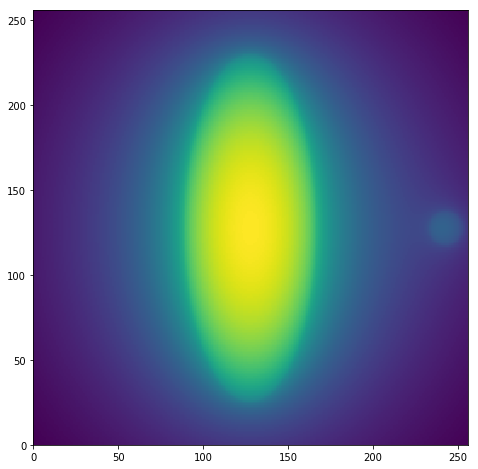
\includegraphics[width=\linewidth]{2_direct_2.png}
    \caption{附件(2)}
    \label{fig:2_direct:2}
  \end{subfigure}%
  \hfill
  \begin{subfigure}[b]{0.3\textwidth}
    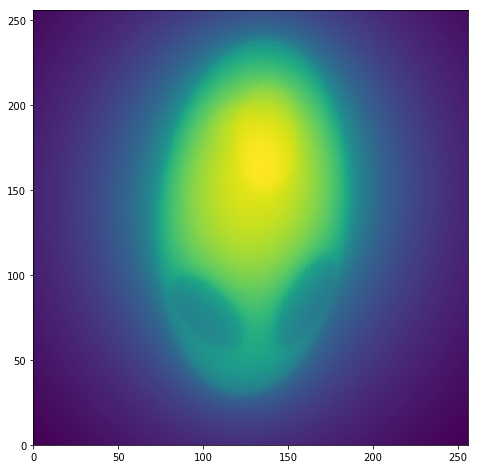
\includegraphics[width=\linewidth]{2_direct_3.png}
    \caption{附件(3)}
    \label{fig:2_direct:3}
  \end{subfigure}%
  \hfill
  \begin{subfigure}[b]{0.3\textwidth}
    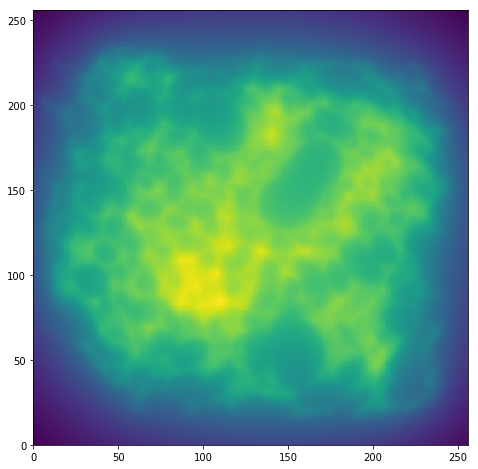
\includegraphics[width=\linewidth]{2_direct_5.png}
    \caption{附件(5)}
    \label{fig:2_direct:5}
  \end{subfigure}

  \caption{直接反投影恢复出的介质}
  \label{fig:2_direct}
\end{figure}

\subsubsection{改进:滤波反投影}
由于直接反投影法的缺陷,根据公式\ref{equ:2_fourier_conv},我们可以通过在进行反投影前对投影数据进行滤波处理以提高结果的准确度。对于每一个旋转角度$\theta$,在遍历像素前先进行以下处理:
\begin{enumerate}
  \item DFT:将接收器坐标点对应的吸收值进行离散 Fourier 变换
  \item 滤波:在上一步所得的频域结果上乘给定的滤波函数
  \item IDFT:将上一部所得的结果进行逆离散 Fourier 变换,并去除所有结果的虚部,只保留实部作为新的吸收值
\end{enumerate}

关于滤波器的选择,许多文献均有比较详细的介绍\cite{gao2010}\pagescite[][96-97]{gu2012}\pagescite[][80-82]{kang2014}。作为测试,我们尝试了R-L滤波器、S-L滤波器、Hanning滤波器等多种不同的函数。由于R-L滤波函数在工业界被广泛使用、原理与实现比较简单、与其他滤波器效果也没有明显劣势,我们将其作为最终的选择。在R-L滤波器算法的实现部分,我们参考了 Matlab 中 \texttt{iradon} 函数的实现\pagescite[][70-76]{kak2001}。

图\ref{fig:2_filter}为对三个附件分别进行滤波反投影得到的图像。从直观上图像的清晰度、辨识度都有了极大的提升。图\ref{fig:2_direct:2}与附件(2)给出的模型吻合度高,完整地恢复出了圆、椭圆的内部,吸收率分布也很均匀。附件(3)(图\ref{fig:2_direct:3})的介质主体形状为一个放置不正的椭圆,内有五个近似椭圆形的吸收率不同的区域:下部两个区域吸收率很低,中部的一个接近介质其他部分,上部的两个吸收率较高,并有重叠(重叠部分为两者吸收率之和)。附件(5)(图\ref{fig:2_direct:5})是一种多孔的稀疏介质,介质的吸收率分布并不均匀。

\begin{figure}[htbp]
  \centering

  \begin{subfigure}[b]{0.3\textwidth}
    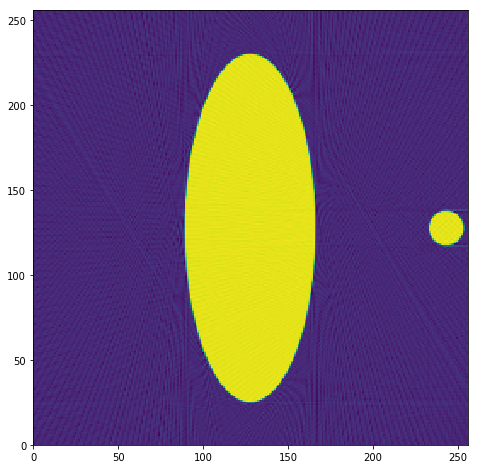
\includegraphics[width=\linewidth]{2_filter_2.png}
    \caption{附件(2)}
    \label{fig:2_filter:2}
  \end{subfigure}%
  \hfill
  \begin{subfigure}[b]{0.3\textwidth}
    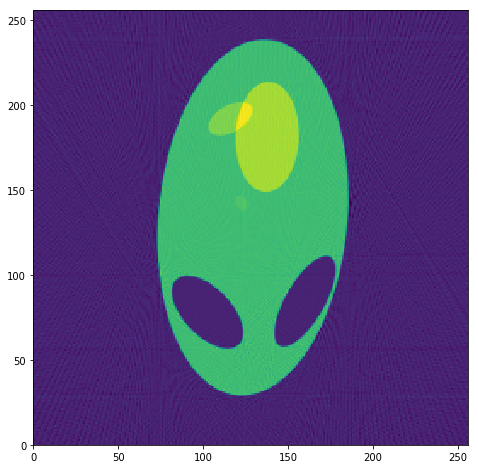
\includegraphics[width=\linewidth]{2_filter_3.png}
    \caption{附件(3)}
    \label{fig:2_filter:3}
  \end{subfigure}%
  \hfill
  \begin{subfigure}[b]{0.3\textwidth}
    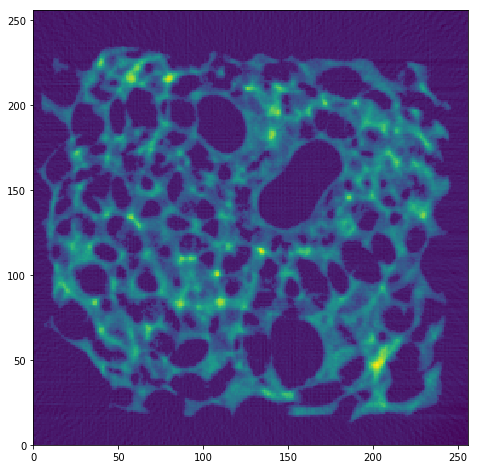
\includegraphics[width=\linewidth]{2_filter_5.png}
    \caption{附件(5)}
    \label{fig:2_filter:5}
  \end{subfigure}

  \caption{滤波反投影恢复出的介质}
  \label{fig:2_filter}
\end{figure}

\subsubsection{最终:计算吸收率}

最终每点的吸收率需要对数据进行归一化:计算重建附件(2)得到的圆与椭圆内部的吸收率平均值(再除$1.00$),此即为在我们恢复得到的一点的数值与题目给出的吸收率的比例因子;根据比例因子即可将样例(2)与(3)的每点数值转化为对应的吸收率。所有的吸收率数据已按照题目要求在附件中给出。

由于题目所给的10个位置在进行坐标转换后并非落在$256 \times 256$坐标的整数点上,故我们需要对每个点的吸收率进行重新计算,以确保数据的准确。计算方法与上面完全是相同的,仅仅将每次遍历的点变为给定的10个。最后我们得到了附录中的表\ref{table:absort_rate}中的结果。由于不可避免的噪声影响与算法的局限性,计算出部分点的吸收值为负;为了符合真实情况,我们将负数结果统一置为$0$。同时我们也将这10个点对应绘制在了图\ref{fig:2_dots}上,以供参考。

\begin{figure}[htbp]
  \centering

  \begin{subfigure}[b]{0.3\textwidth}
    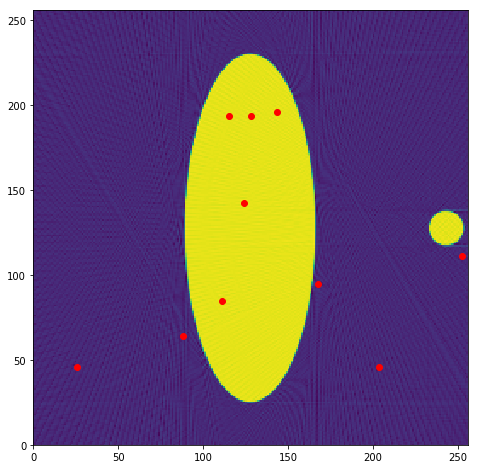
\includegraphics[width=\linewidth]{2_dots_2.png}
    \caption{附件(2)}
    \label{fig:2_dots:2}
  \end{subfigure}%
  \hfill
  \begin{subfigure}[b]{0.3\textwidth}
    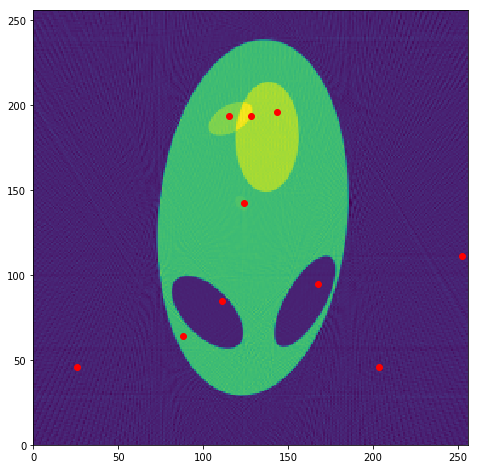
\includegraphics[width=\linewidth]{2_dots_3.png}
    \caption{附件(3)}
    \label{fig:2_dots:3}
  \end{subfigure}%
  \hfill
  \begin{subfigure}[b]{0.3\textwidth}
    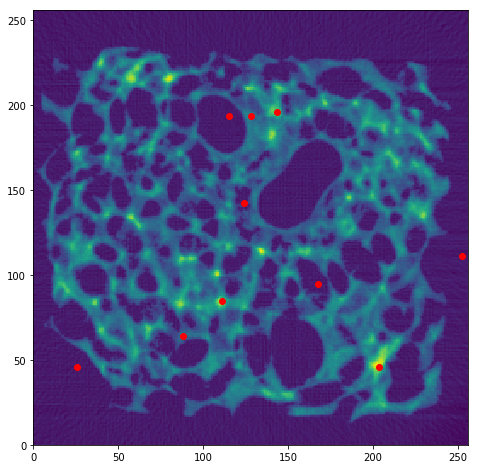
\includegraphics[width=\linewidth]{2_dots_5.png}
    \caption{附件(5)}
    \label{fig:2_dots:5}
  \end{subfigure}

  \caption{恢复出的图像上给定的坐标点}
  \label{fig:2_dots}
\end{figure} 

\subsection{问题4}

\subsubsection{精度与稳定性分析}
问题4要求分析问题1中参数标定的精度和稳定性,下面逐一进行讨论。

首先考虑求解接收器间距$l$时使用的回归方法的精度。我们可以认为由于外界干扰以及机器自身的内禀影响,测量得到的值 $L_m$ 与真实值 $\hat L_m$ 之间有如下关系:

\begin{equation}
	L_m = \hat L_m + \sigma\varepsilon_m\text{, } \varepsilon_m \sim \mathcal N(0, 1)
	\label{equ:4_relation}
\end{equation}

并且$\varepsilon_0, \varepsilon_1, \cdots, \varepsilon_n$之间相互独立。

那么对于公式$\ref{equ:1_reg}$中右侧量$L_0^2-L_m^2$可以计算其方差:

\begin{equation}
	\begin{aligned}
		\var[L_0^2-L_m^2] &= \var[(\hat L_0 + \sigma\varepsilon_0)^2] + \var[(\hat L_m - \sigma\varepsilon_m)^2] \\
		&\leq \var[2\sigma\varepsilon_0] + \var[\sigma^2\varepsilon_0^2] + \var[2\sigma\varepsilon_m] + \var[\sigma^2\varepsilon_m^2] \\
		&= 8\sigma^2 + 4\sigma^4
	\end{aligned}
	\label{equ:4_reg_var}
\end{equation}

如果利用$l_0, \cdots, l_n$共$n + 1$条直线来计算接收器间隔$l$,将公式$\ref{equ:1_reg}$中的回归方程记为$Ax=L$,其中$L=\frac{1}{4}(L_0^2-L_1^2, \cdots, L_0^2 - L_n^2)^T$,$x = ((D_0-R)l, l^2)^T$,并且$x = (A^TA)^{-1}A^TL$,计算可得

\begin{equation}
	(A^TA)^{-1} =
	\begin{bmatrix}
		\frac{9}{2 \left(n^2+n-2\right)} & -\frac{6 (2 n+1)}{n (n+1) \left(n^2+n-2\right)} \\
		-\frac{6 (2 n+1)}{n (n+1) \left(n^2+n-2\right)} & \frac{36}{n (n+1) \left(n^2+n-2\right)} \\
	\end{bmatrix}
	\label{equ:4_ATA_reg}
\end{equation}

为了符号简便,将矩阵\ref{equ:4_ATA_reg}第二行记为$(a_{21}, a_{22})$,可以得到

\begin{equation}
	\begin{aligned}
		\var[l^2] &\leq \var[a_{21}\sum_{i=1}^n 2iL_i] + \var[a_{22} \sum_{i=1}^ni^2L_i] \\
		&\leq \frac{2\sigma^2 + \sigma^4}{4}\left[ a_{21}^2 P_3(n) + a_{22}^2 P_5(n) \right] \\
		&=\frac{2\sigma^2 + \sigma^4}{Q_3(n)}
\end{aligned}
	\label{equ:4_var_finite}
\end{equation}

其中 $P_3(n), P_5(n)$ 分别是关于$n$的$3$次多项式和$5$次多项式,$Q_3(n)$是关于$n$的$3$次多项式。因此,我们知道$\var[l^2]$和$n$至少为立方反比关系。

\begin{figure}[htbp]
  \centering

  \begin{subfigure}[b]{0.3\textwidth}
    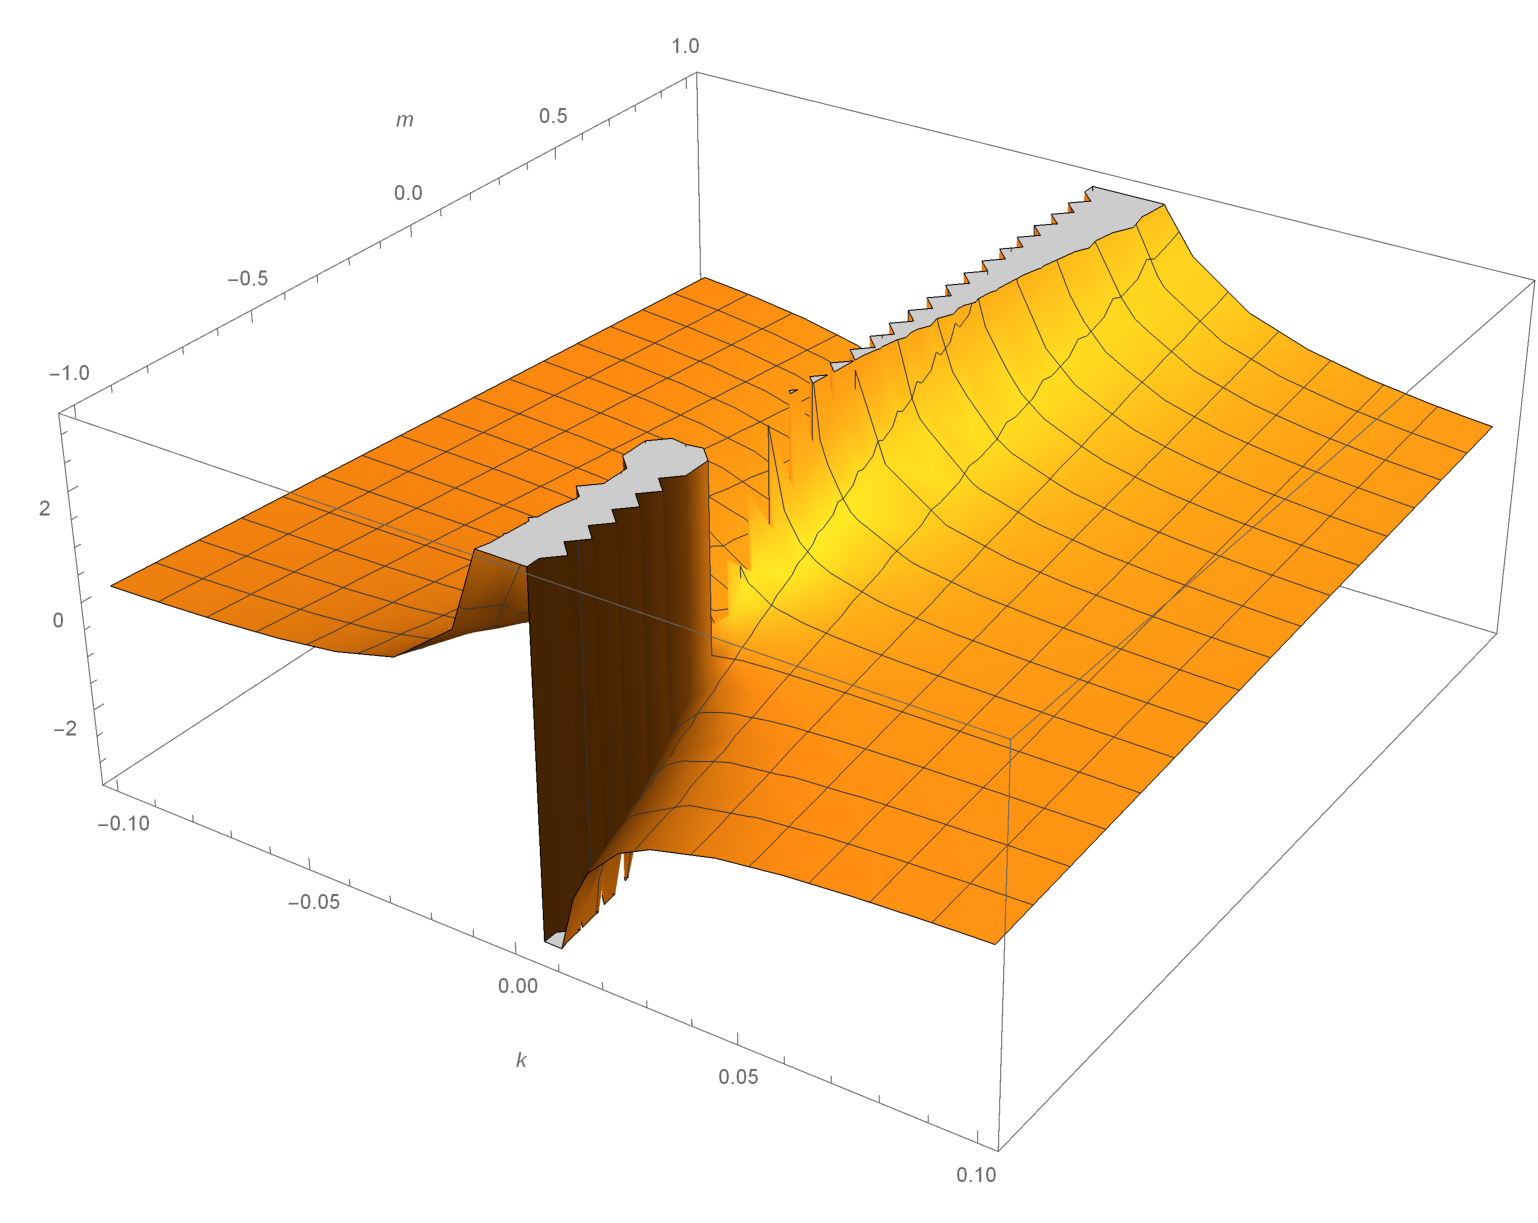
\includegraphics[width=\linewidth]{4_slope_fault_2.pdf}
    \caption{$\displaystyle \frac{\partial k}{\partial L_0}, |k| \leq 0.1 $}
    \label{fig:4_slope_fault:1}
  \end{subfigure}%
  \hfill
  \begin{subfigure}[b]{0.3\textwidth}
    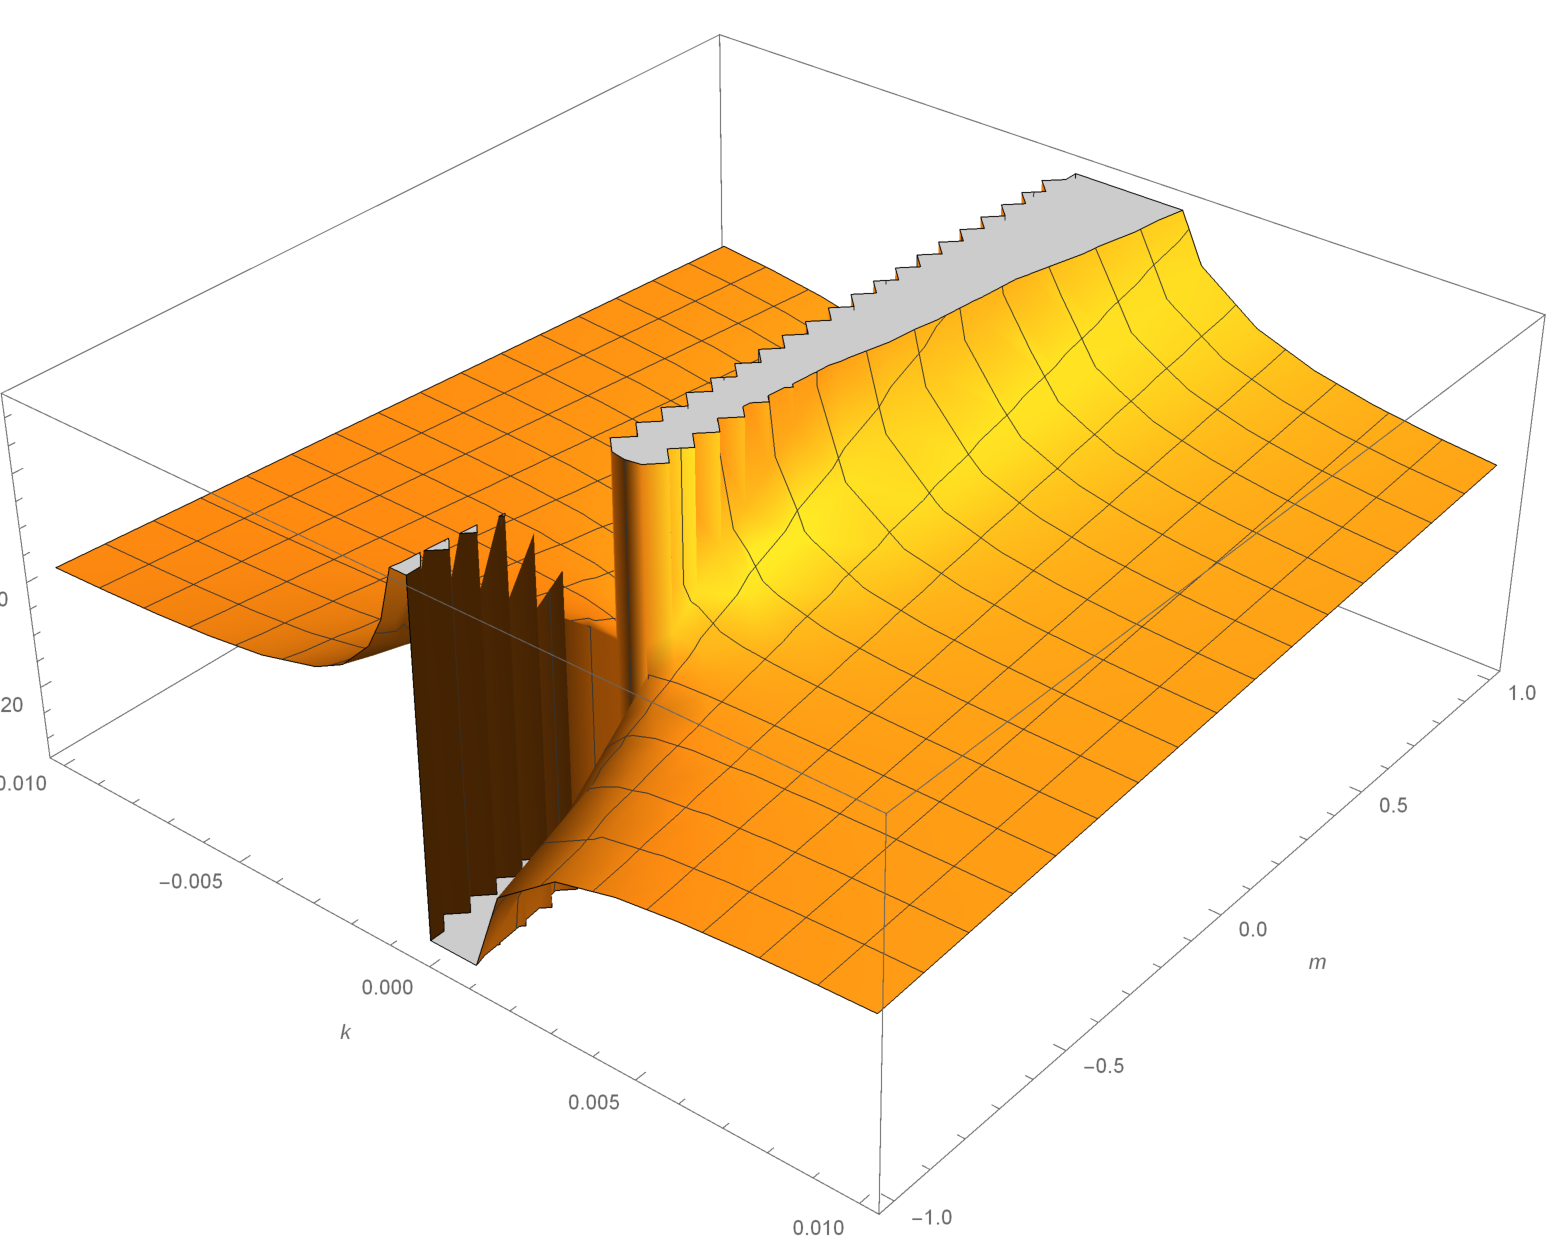
\includegraphics[width=\linewidth]{4_slope_fault.pdf}
    \caption{$\displaystyle \frac{\partial k}{\partial L_0}, |k| \leq 0.01 $}
    \label{fig:4_slope_fault:2}
  \end{subfigure}%
  \hfill
  \begin{subfigure}[b]{0.3\textwidth}
    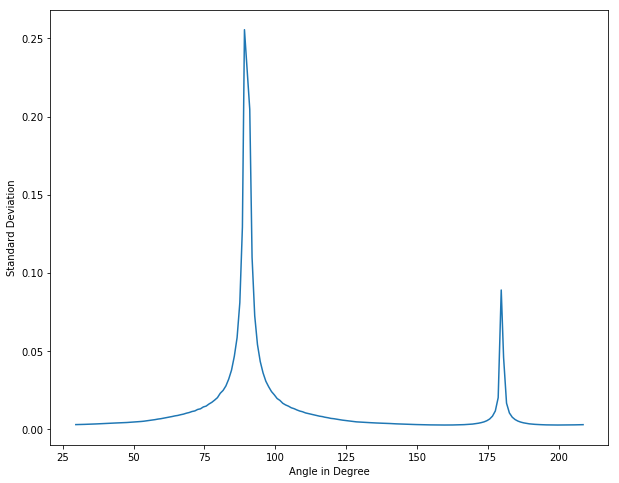
\includegraphics[width=\linewidth]{4_std_err_degree.png}
    \caption{计算得到$\omega$的标准差}
    \label{fig:4_std_err_degree}
  \end{subfigure}

  \caption{图\subref{fig:4_slope_fault:1}与图\subref{fig:4_slope_fault:2}是当$k$在不同范围内变化时,可以观察到当$k \to 0$时,$\displaystyle \frac{\partial k}{\partial L_0} \to \infty$;由图\subref{fig:4_std_err_degree}可见当椭圆轴与射线接近平行时计算得到的$\omega$标准差有突增}
  \label{fig:4_analysis}
\end{figure} 

对于角度的计算,我们是通过方程组\ref{equ:1_degree_full}中联立相邻两个方程再取平均来完成的。如图\ref{fig:4_std_err_degree},在投影线和椭圆的轴接近平行时标准差较大,下面将会分析该现象发生的原因。

首先将方程\ref{equ:1_degree_full}中的弦长写成关于$m_0$和$\omega$的函数$G_i(\omega, m_0) = G_i(\arctan k, m_0)$。为了方便,我们不妨设联立的两个方程为

\begin{equation}
	\left\{
		\begin{aligned}
			G_0(\omega, m_0) &= L_0 \\
			G_i(\omega, m_0) &= L_i
		\end{aligned}
	\right.
	\label{equ:5_length_eq2}
\end{equation}

根据反函数定理,如果$\partial (L_0, L_i) / \partial (\omega, m_0)$存在,那么

\begin{equation}
	\frac{\partial(\omega, m_0)}{\partial(L_0, L_i)}
	= \left[\frac{\partial(L_0, L_i)}{\partial(\omega, m_0)}\right]^{-1}
	= \left[\frac{\partial(L_0, L_i)}{\partial(k, m_0)}\cdot \frac{\partial(k, m_0)}{\partial(\omega, m_0)}\right]^{-1}
	\label{equ:5_inv_partial}
\end{equation}

记 $\displaystyle J_\omega(\omega, m_0) = \frac{\partial(L_0, L_i)}{\partial(\omega, m_0)}$,$\displaystyle J_k(k, m_0) = \frac{\partial(L_0, L_i)}{\partial(k, m_0)}$,从公式\ref{equ:1_degree_full}可以看出$J_\omega(\omega, m_0)$的各个元素在原点附近都是连续可微的。并且计算后可得

\begin{equation}
	J_\omega(0, m_0) = J_k(0, m_0) = \begin{bmatrix}
		0 & -\frac{2 a m_0}{b \sqrt{b^2 - m_0^2}} \\
		0 & -\frac{2 a (i l+m_0)}{b \sqrt{b^2 - (i l+m_0)^2}} \\
	\end{bmatrix},
	\label{equ:5_jacob_k0}
\end{equation}

我们可以设

\begin{equation}
	J_\omega(\omega, m_0) = \begin{bmatrix}
		A(\omega, m_0) & B(\omega, m_0) \\
		C(\omega, m_0) & D(\omega, m_0)
	\end{bmatrix}
	\label{equ:5_j_omega}
\end{equation}

这样当 $\det J_\omega$ 非零时,该矩阵可逆并且

\begin{equation}
	J_\omega^{-1}(\omega, m_0) = \frac{1}{\det J_\omega(\omega, m_0)}
	\begin{bmatrix}
		D(\omega, m_0) & -B(\omega, m_0) \\
		-C(\omega, m_0) & A(\omega, m_0)
	\end{bmatrix}
	\label{equ:5_j_omega_inv}
\end{equation}

由公式\ref{equ:5_jacob_k0}以及$A, B, C, D$的连续性可知,当$\omega \to 0$时,$A \to 0$且$C \to 0$。而此时,根据$m_0$的几何意义可知$|m_0| < b$,不妨认为在选取数据时忽略距离椭圆边界最近的两条直线,那么$B, D$在原点附近有界。因此可以得到

\begin{equation}
	\det J_\omega(\omega, m_0) = AD - BC \to 0
	\label{equ:5_det_to_0}
\end{equation}

那么就有

\begin{equation}
	\frac{\partial \omega}{\partial L_0} = \frac{D(\omega, m_0)}{\det J_\omega(\omega, m_0)}  \to \infty,\quad\quad
	\frac{\partial \omega}{\partial L_i} = \frac{D(\omega, m_0)}{\det J_\omega(\omega, m_0)}  \to \infty
	\label{equ:5_partial_to_inf}
\end{equation}

这样,根据\ref{equ:4_relation},在存在一个白噪声$\varepsilon\sim\mathcal N(0, \sigma^2)$的情况下,当投影线与椭圆的轴平行的时候所求得的$\omega$的方差将会过大。相应地,$\theta$的方差也变大。

综上,我们得到如下的分析结果:
\begin{principle}
\label{prcp:l_n}
回归得到的$l$精确程度与穿过圆区域的射线数目成正相关
\end{principle}

\begin{principle}
\label{prcp:omega}
当射线与椭圆的轴接近平行时,随机噪声的存在将使$\theta$的求解结果变得不稳定
\end{principle}

最后,由于旋转中心的坐标可$C(X_0,Y_0)$完全由上述求得的$l$与$\theta$所确定,故其精度与稳定性受到上述两个因素的共同制约。


\subsubsection{模板设计与模型修正}

下面提出一个简单的模板设计来减轻上述问题对标定产生的影响。

对于定律\ref{prcp:l_n}的结论,已知增大穿过圆的射线条数$n$能够增加$l$的精确程度。由于接收器间隔是一定的,故应当增大模型上圆形区域的尺寸。对于定律\ref{prcp:omega}的结论,我们应当尽量避开射线与椭圆轴平行的角度(至多有三个位置),故可以每次扫描后将椭圆模板绕其中心旋转一定角度,重复多次这样的操作,就能获取充分多的数据避开“坏”的角度。

本参数标定模型的模板包含一至多个半径不同的圆与一个椭圆,并且其吸收率均相同(如1.0000)。在每次扫描时均只使用其中的一个,避免扫描条带出现重叠现象影响数据的处理。

对于接收器间距$l$的计算,可选取半径较大的圆(可以考虑直径为托盘宽度的$2/3$),圆心与托盘中心重合,再利用第\ref{sec:1_calc_l}节提出的回归算法计算$l$。如果认为方差过大或者精度不足可以改变圆的位置或半径多次计算并且取平均值。$l$值的计算与圆心所处的位置无关。

对于探测系统相对于初始状态旋转角度$\theta$的计算,选取中心位于托盘中心的,长轴长约为托盘宽度$2/3$且与x轴平行的椭圆。设$n$为总共的扫描次数(一般推荐取5左右),则每次椭圆旋转的角度应为$\pi/n$。假设第$i$扫描得到的第$j$个旋转角度的估计值为$\theta_{i,j}$,数据的标准差为$s_{i,j}$,且$\alpha_i = \argmin_j s_{i,j}$,则最后确定的旋转角度$\theta_i$为$\theta_{i, \alpha_i}$。 

\section{模型评价与展望}
在这次建模过程中,我们成功完成了题目所要求的标定系统参数与重建扫描图像的任务,并定量分析原有模型的不足,提出了在理论上更优的标定模型。

我们的整体工作突出之处有:
\begin{itemize}
  \item 在标定参数的过程中充分利用题目给出的数据与几何关系构成方程,求解得到的参数值较精确,统计意义上较为优秀
  \item 在重建图像的过程中选择了恰当的投影方法与滤波函数,恢复出的图像轮廓清晰,在样本上的恢复与原数据吻合程度较高
  \item 在模型分析过程中充分考虑可能的测量误差,定量地建立了样本数量、系统状态与误差间的数学关系
  \item 提出的新模型在标定过程中使用的算法较简单,且得到的数据精度更高
\end{itemize}

不足之处有:
\begin{itemize}
  \item 求解参数过程使用的关系式较为复杂,且数据量大,导致求解过程略显缓慢
  \item 使用的R-L滤波函数会在空域中造成震荡响应,降低了吸收率较低的介质区域的信噪比
  \item 提出的新模型需要较多次扫描得到的数据,操作较为繁琐,且对模板放置位置精度要求较高
\end{itemize}

此模型未来可能有的进一步发展包括且不限于:
\begin{itemize}
  \item 调整算法以适应接收器间距不再严格相等的情况,消除系统带来的误差
  \item 考虑射线在空气等非被测介质中的损耗及可能的散射、反射等现象带来的干扰
  \item 将标定与重建算法从二维空间推广到三维甚至更高维度(含时)的空间
  \item 优化计算复杂度,减少待解方程数量,将数值运算问题转化为较易解决的统计学问题
\end{itemize}

\nocite{*}

\printbibliography[heading=bibliography,title=参考文献]
\addcontentsline{toc}{section}{参考文献}

\clearpage

\renewcommand{\theHsection}{A\arabic{section}}
\appendix
\section{建模结果数据}

\begin{table}[htbp]
\centering
\caption{计算出的数值结果}
\label{table:values}
\begin{tabular}{@{}lll@{}}
\toprule
符号          & 值     &   说明         \\ \midrule
$l$    & $0.2766\,\si{mm}$     & 两个相邻接收器间的距离                  \\
$(x_0, y_0)$ & $(-9.2383\,\si{mm}, 6.2663\,\si{mm})$  & $xoy$坐标系中探测系统旋转中心坐标 \\ \bottomrule
\end{tabular}
\end{table} 

\begin{longtable}{@{}cccccc@{}}
\caption{180个旋转方向}
\label{table:roration_degrees}
\endfirsthead
\endhead
\hline
$29.6422^\circ$ & $30.9957^\circ$ & $31.5511^\circ$ & $32.6404^\circ$ & $33.6726^\circ$ & $34.6418^\circ$\\ \hline
$35.6417^\circ$ & $36.6416^\circ$ & $37.6415^\circ$ & $38.6414^\circ$ & $39.6412^\circ$ & $40.6411^\circ$\\ \hline
$41.6410^\circ$ & $42.6409^\circ$ & $43.6408^\circ$ & $44.7911^\circ$ & $45.6406^\circ$ & $46.6406^\circ$\\ \hline
$47.6405^\circ$ & $48.6404^\circ$ & $49.6403^\circ$ & $50.6402^\circ$ & $51.6402^\circ$ & $52.6400^\circ$\\ \hline
$53.6399^\circ$ & $54.6396^\circ$ & $55.6393^\circ$ & $56.6389^\circ$ & $57.6386^\circ$ & $58.6382^\circ$\\ \hline
$59.6379^\circ$ & $60.5365^\circ$ & $61.6370^\circ$ & $62.6364^\circ$ & $63.6360^\circ$ & $64.6353^\circ$\\ \hline
$65.6349^\circ$ & $66.6342^\circ$ & $67.6335^\circ$ & $68.6327^\circ$ & $69.6320^\circ$ & $70.6309^\circ$\\ \hline
$71.6300^\circ$ & $72.6288^\circ$ & $73.6276^\circ$ & $74.6262^\circ$ & $75.6247^\circ$ & $76.6228^\circ$\\ \hline
$77.6208^\circ$ & $78.6183^\circ$ & $79.6154^\circ$ & $80.6119^\circ$ & $81.6075^\circ$ & $82.6019^\circ$\\ \hline
$83.5949^\circ$ & $84.5856^\circ$ & $85.5718^\circ$ & $86.5496^\circ$ & $87.5109^\circ$ & $88.4265^\circ$\\ \hline
$89.1500^\circ$ & $91.0183^\circ$ & $91.8326^\circ$ & $92.7671^\circ$ & $93.7351^\circ$ & $94.7164^\circ$\\ \hline
$95.7041^\circ$ & $96.6950^\circ$ & $97.6888^\circ$ & $98.6838^\circ$ & $99.6795^\circ$ & $100.6763^\circ$\\ \hline
$101.6735^\circ$ & $102.6712^\circ$ & $103.6692^\circ$ & $104.6676^\circ$ & $105.6659^\circ$ & $106.6646^\circ$\\ \hline
$107.6633^\circ$ & $108.6624^\circ$ & $109.6613^\circ$ & $110.6606^\circ$ & $111.6595^\circ$ & $112.6588^\circ$\\ \hline
$113.6582^\circ$ & $114.6575^\circ$ & $115.6570^\circ$ & $116.6564^\circ$ & $117.4534^\circ$ & $118.6554^\circ$\\ \hline
$119.6549^\circ$ & $120.6546^\circ$ & $121.6543^\circ$ & $122.6538^\circ$ & $123.6535^\circ$ & $124.6532^\circ$\\ \hline
$125.6529^\circ$ & $126.6526^\circ$ & $127.6524^\circ$ & $128.6523^\circ$ & $129.6521^\circ$ & $130.6521^\circ$\\ \hline
$131.7520^\circ$ & $132.6519^\circ$ & $133.6519^\circ$ & $134.6518^\circ$ & $135.6517^\circ$ & $136.6517^\circ$\\ \hline
$137.6516^\circ$ & $138.6515^\circ$ & $139.6514^\circ$ & $140.6513^\circ$ & $141.6511^\circ$ & $142.6510^\circ$\\ \hline
$143.6509^\circ$ & $144.6508^\circ$ & $145.6507^\circ$ & $146.6507^\circ$ & $147.6505^\circ$ & $148.6505^\circ$\\ \hline
$149.6504^\circ$ & $150.6503^\circ$ & $151.6502^\circ$ & $152.6502^\circ$ & $153.6501^\circ$ & $154.6501^\circ$\\ \hline
$155.6501^\circ$ & $156.6500^\circ$ & $157.6500^\circ$ & $158.6500^\circ$ & $159.6500^\circ$ & $160.6500^\circ$\\ \hline
$161.6500^\circ$ & $162.6500^\circ$ & $163.6501^\circ$ & $164.6501^\circ$ & $165.6503^\circ$ & $166.6503^\circ$\\ \hline
$167.6506^\circ$ & $168.6508^\circ$ & $169.6510^\circ$ & $170.6513^\circ$ & $171.6517^\circ$ & $172.6523^\circ$\\ \hline
$173.6530^\circ$ & $174.6541^\circ$ & $175.6556^\circ$ & $176.6584^\circ$ & $177.6633^\circ$ & $178.6757^\circ$\\ \hline
$179.7497^\circ$ & $180.5807^\circ$ & $181.6219^\circ$ & $182.6311^\circ$ & $183.6351^\circ$ & $184.6373^\circ$\\ \hline
$185.6387^\circ$ & $186.6397^\circ$ & $187.6404^\circ$ & $188.6409^\circ$ & $189.6413^\circ$ & $190.6416^\circ$\\ \hline
$191.6419^\circ$ & $192.6421^\circ$ & $193.6422^\circ$ & $194.6423^\circ$ & $195.6424^\circ$ & $196.6425^\circ$\\ \hline
$197.6425^\circ$ & $198.6425^\circ$ & $199.6425^\circ$ & $200.6425^\circ$ & $201.6425^\circ$ & $202.6425^\circ$\\ \hline
$203.6425^\circ$ & $204.6424^\circ$ & $205.6424^\circ$ & $206.6424^\circ$ & $207.6423^\circ$ & $208.6317^\circ$\\ \hline
\end{longtable}

\begin{figure}[htbp]
  \centering
  \begin{subfigure}[b]{0.3\textwidth}
    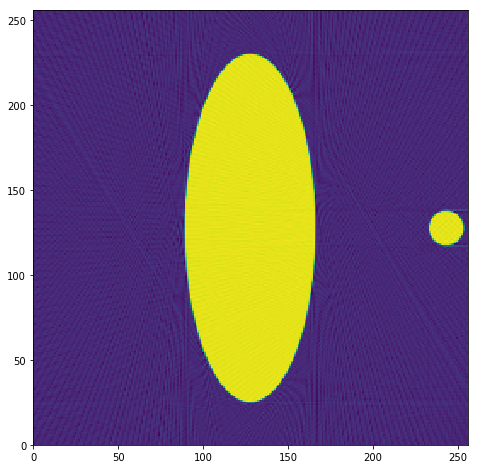
\includegraphics[width=\linewidth]{2_filter_2.png}
    \caption{附件(2)}
  \end{subfigure}%
  \hfill
  \begin{subfigure}[b]{0.3\textwidth}
    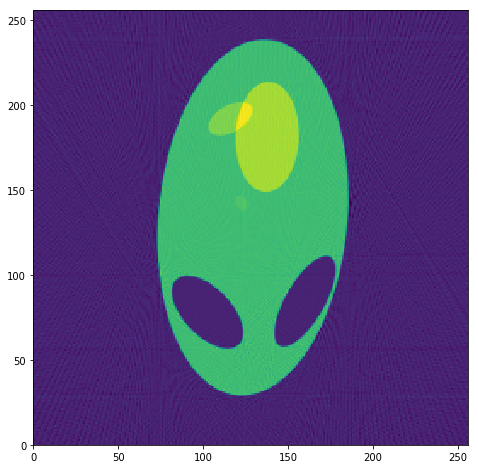
\includegraphics[width=\linewidth]{2_filter_3.png}
    \caption{附件(3)}
  \end{subfigure}%
  \hfill
  \begin{subfigure}[b]{0.3\textwidth}
    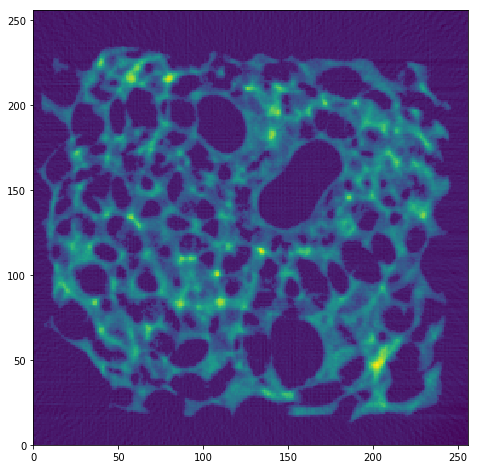
\includegraphics[width=\linewidth]{2_filter_5.png}
    \caption{附件(5)}
  \end{subfigure}
  \caption{滤波反投影恢复出的介质}
  \label{fig:4_filter_copy}
\end{figure}

\begin{table}[htbp]
\centering
\caption{两样例给定点处的吸收率数据}
\label{table:absort_rate}
\begin{tabular}{@{}cccccc@{}}
\toprule
      & 1         & 2        & 3         & 4        & 5  \\ \midrule	
附件(3) & $0$ & $0.9979$ & $0$ & $1.2050$ & $1.0866$ \\
附件(5) & $0.0780$  & $2.8227$ & $6.7965$  & $0.1994$ & $0.1626$ \\ \bottomrule
      & 6         & 7        & 8         & 9        & 10  \\ \midrule
附件(3)& $1.4175$ & $1.2915$ & $0.0064$  & $0.0286$ & $0$ \\
附件(5)& $3.1407$ & $6.4676$ & $0$ & $7.3136$ & $0$ \\ \bottomrule
\end{tabular}
\end{table}
\clearpage
\section{程序源码}

\emph{注:所有的Python代码需要在交互式环境(如Jupyter Notebook)中顺序依次执行。}

\subsection{Python(第一部分)}
此部分主要完成的工作为读入数据,使用条带未重合部分进行回归得到圆半径和圆心的精确投影坐标。后将每个旋转角度的数据输出待Mathematica计算。

\begin{minted}[frame=lines, linenos=true, breaklines=true]{python}
#!/use/bin/env python3
# -*- coding: utf8 -*-

import matplotlib.pyplot as plt
import copy
import numpy as np
import scipy.stats
from sklearn import linear_model
import math
import re
import fileinput

def load_data(filename):
    f = open(filename, 'r').read()
    return [list(map(float, s.split('\t')))
            for s in f.replace(' ', '').strip().split('\n')]

attach_1 = load_data('attachment1.txt')
attach_2 = load_data('attachment2.txt')
attach_3 = load_data('attachment3.txt')
attach_5 = load_data('attachment5.txt')

# Question 1
data1 = np.array(attach_2)
data1 = np.transpose(data1)

# find the position of the circle in the first scanline
for i in range(511, 0, -1):
    if data1[0][i] != 0:
        circle_bottom = i
        break

for i in range(circle_bottom, 0, -1):
    if data1[0][i] == 0:
        circle_top = i + 1
        break

circle = [(circle_top, circle_bottom)]
circle_shift = 5

for i in range(1, 120):
    ct, cb = circle[-1]
    # find circle top
    max_now, max_id = -1, 999
    for shift in range(1, circle_shift):
        val = data1[i][ct - shift] - data1[i][ct - shift - 1]
        if val > max_now:
            max_id, max_now = ct - shift, val
    ct = min(max_id, ct)

    # find circle bottom
    max_now, max_id = -1, 999
    for shift in range(1, circle_shift):
        val = data1[i][cb - shift - 1] - data1[i][cb - shift]
        if val > max_now:
            max_id, max_now = cb - shift, val
    cb = min(max_id, cb)

    circle.append((ct, cb))

for i in range(120, 180):
    for j in range(0, 512):
        if data1[i][j] != 0:
            ct = j
            break
    for j in range(ct, 512):
        if data1[i][j] == 0:
            cb = j - 1
            break
    circle.append((ct, cb))

def find_bottom(data, start):
    for i in range(start, 0, -1):
        if data[i] != 0:
            return i

ellipse_shift = 5
ellipse_bottom = [find_bottom(data1[0], 390)]

for i in range(1, 30):
    eb = ellipse_bottom[-1]
    # find circle bottom
    max_now, max_id = -1, 0
    for shift in range(1, circle_shift):
        val = data1[i][eb + shift - 1] - data1[i][eb + shift]
        if val > max_now:
            max_id, max_now = eb + shift - 1, val
    ellipse_bottom.append(max(max_id, eb))

for i in range(30, 180):
    ellipse_bottom.append(find_bottom(data1[i], 511))

def find_top(data, start):
    for i in range(start, 512):
        if data[i] != 0:
            return i

ellipse_top = [find_top(data1[i], 0) for i in range(85)]

for i in range(85, 120):
    et = ellipse_top[-1]
    # find circle top
    max_now, max_id = -1, 0
    for shift in range(0, circle_shift):
        val = data1[i][et + shift] - data1[i][et + shift - 1]
        if val > max_now:
            max_id, max_now = et + shift, val
    ellipse_top.append(max(max_id, et))

ellipse_top.extend([find_top(data1[i], 120) for i in range(120, 180)])

# output to file
open('bound-circle.txt', 'w').write('\n'.join(
    [str(c[0]) + '\t' + str(c[1]) for c in circle]))
open('bound-ellipse.txt', 'w').write('\n'.join(
    [str(ellipse_top[i]) + '\t' + str(ellipse_bottom[i]) for i in range(180)]))

# scanline width
def get_circle_scanline(i):
    return data1[i][circle[i][0]:circle[i][1] + 1]

def scanline_width(line):
    n = len(line)
    y = [0.25 * (line[0] * line[0] - line[i] * line[i]) for i in range(1, n)]
    X = [(2 * i, i * i) for i in range(1, n)]
    clf = linear_model.LinearRegression()
    clf.fit(X, y)
    _, LL = clf.coef_
    return math.sqrt(LL)

l_i_many = [scanline_width(get_circle_scanline(i)) for i in range(110, 180)]
l_i = np.mean(l_i_many)

d_i_many = [max(get_circle_scanline(i)) for i in range(110, 180)] \
         + [max(get_circle_scanline(i)) for i in range(0, 14)]
d_i = max(d_i_many)
d_s = d_i / l_i  # circle radius in scanline

def find_bound_s(index, ignore=2):
    cb, ct = circle[index]
    line = data1[index]
    circle_line = line[cb : ct + 1]
    peak = np.argmax(circle_line)

    d_center_s = [0.5 * math.sqrt(d_i * d_i - l * l) / l_i for l in circle_line]

    center_many = []
    for i, dc_s in enumerate(d_center_s[: peak - ignore]):
        center_many.append(cb + i + dc_s)

    for i, dc_s in enumerate(d_center_s[peak + ignore + 1: ]):
        base = cb + i + peak + ignore + 1
        center_many.append(base - dc_s)

    center_s = np.mean(center_many)
 #   print(np.var(center_many))

    return center_s - 0.5 * d_s, center_s + 0.5 * d_s

bound_0_13 = [find_bound_s(i) for i in range(13)]
bound_110_180 = [find_bound_s(i) for i in range(110, 180)]

def get_angle(width):
    D = d * width
    s = 2880/11 * (1/225 - 4/(D**2))
    t = math.asin(s)
    n2 = math.atan(math.sqrt((4*40*40-D**2)/(D**2-4*15*15)))
    return n2 * 180 / math.pi

open('middle_0_13.txt', 'w').write('\n'.join([str(0.5 * (y + x)) for x, y in bound_0_13]))
open('middle_110_180.txt', 'w').write('\n'.join([str(0.5 * (y + x)) for x, y in bound_110_180]))

def extract_ellipse(index, ignore=3):
    et, eb = ellipse_top[index] + ignore, ellipse_bottom[index] - ignore
    ct, cb = circle[index]
    ct, cb = ct - ignore, cb + ignore

    line = data1[index]
    scan_lines = []
    for e in range(et, eb):
        if ct <= e <= cb or not line[e]:
            continue
        scan_lines.append((e - et, line[e]))
    return scan_lines

ellipse_slines = [extract_ellipse(i) for i in range(180)]

def write_ellipse_to_file(filename, line_id):
    f = open(filename, 'w')
    f.write('\n'.join(str(n) + ' ' + str(L) for n, L in ellipse_slines[line_id]))
    f.close()

for i in range(180):
    write_ellipse_to_file('ellipse_scanline/%d.txt' % i, i)

# waiting for Mathematica's output
input('Waiting for Mathematica\' Output')
\end{minted} 


\subsection{Mathematica(第一部分)}
此部分的作用为读入Python初步处理后的数据,并计算每个状态对应的方程解,输出为直线斜率$k$。

\begin{minted}[frame=lines, linenos=true, breaklines=true]{wolfram}
SolveDirection[id_, step_] := (
  equation = ( -L +
         Sqrt[1 + k^2]
           Sqrt[(4 a^4 k^2 m^2)/(b^2 + a^2 k^2)^2 - (
           4 a^2 (-b^2 + m^2))/(b^2 + a^2 k^2)]) /. a -> 26.58675 /.
      b -> 70.898 /. m -> (Subscript[m, 0] + n*l*Sqrt[1 + k^2]) /.
    l -> 0.49029825753407719;
  dirPath = "ellipse_scanline/";
  filePath = dirPath <> ToString[id] <> ".txt";
  data = Import[filePath, "Table"];
  length = Length[data];
  result =
   Table[NSolve[(equation /. n -> data[[i]][[1]] /.
          L -> data[[i]][[2]]) ==
        0 && (equation /. n -> data[[i + step]][[1]] /.
          L -> data[[i + step]][[2]]) == 0, {Subscript[m, 0], k},
      Reals] // Values, {i, Range[1, length - step]}];
  Export[dirPath <> "ans_step_" <> ToString[step] <> "" <>
    ToString[id] <> ".txt", result, "Table"];
  );


SolveDirectionInverted[id_, step_] := (
  equation = (-L +
         Sqrt[1 + p^2]
           Sqrt[(4 b^4 p^2 q^2)/(a^2 + b^2 p^2)^2 - (
           4 b^2 (-a^2 + q^2))/(a^2 + b^2 p^2)]) /. a -> 26.58675 /.
      b -> 70.898 /. q -> (Subscript[q, 0] + n*l*Sqrt[1 + p^2]) /.
    l -> 0.49029825753407719;
  dirPath = "ellipse_scanline/";
  filePath = dirPath <> ToString[id] <> ".txt";
  data = Import[filePath, "Table"];
  length = Length[data];
  result =
   Table[NSolve[(equation /. n -> data[[i]][[1]] /.
          L -> data[[i]][[2]]) ==
        0 && (equation /. n -> data[[i + step]][[1]] /.
          L -> data[[i + step]][[2]]) == 0, {Subscript[q, 0], p},
      Reals] // Values, {i, Range[1, length - step]}];
  Export[dirPath <> "ans_inverted_step_" <> ToString[step] <> "/" <>
    ToString[id] <> ".txt", result, "Table"];
  );

For[i = 0, i < 138, ++i, SolveDirection[i, 1]];

For[i = 138, i < 162, ++i, SolveDirectionInverted[i, 1]];

For[i = 162, i < 180, ++i, SolveDirection[i, 1]];
\end{minted}


\subsection{Python(第二部分)}
本部分读入上一部分的数据后将其转化为准确的弧度值$\theta$,并将其与每一个状态的圆心投影坐标再次输出。
\begin{minted}[frame=lines, linenos=true, breaklines=true]{python}
def load_angle_data(filename):
    slope_many = []
    for line in open(filename, 'r').read().split('\n'):
        if line.strip():
            slope_one_many = re.findall(r'\{-?\d*\.?\d*, (-?\d*\.?\d*)\}', line)
            slope_many.append(abs(float(slope_one_many[0])))
    return slope_many

def calc_angle(index):
    if 138 <= index <= 161:
        is_inverted = True
        filename = 'ellipse_scanline/ans_inverted_step_1/%d.txt'
    else:
        is_inverted = False
        filename = 'ellipse_scanline/ans_step_1/%d.txt'
    slope_many = load_angle_data(filename % index)
    if not slope_many: return 0
    slope = np.mean(slope_many)
    omega = math.pi / 2 - math.atan(slope) if is_inverted else math.atan(slope)
    if index <= 60: theta = math.pi / 2 - omega
    elif index <= 150: theta = math.pi / 2 + omega
    else: theta = 3 * math.pi / 2 - omega
    return theta, np.std(np.arctan(slope_many))

angles = [ calc_angle(i)[0] * 180 / math.pi for i in range(180) ]

angle_f = open('angle_middle_0_13.txt', 'w')
angle_f.write('\n'.join([str(angles[i]) + ' ' + str((bound_0_13[i][1] + bound_0_13[i][0] - 511) / 2) for i in range(13)]))
angle_f.close()
angle_f = open('angle_middle_110_180.txt', 'w')
angle_f.write('\n'.join([str(angles[i]) + ' ' + str((bound_110_180[i - 110][1] + bound_110_180[i - 110][0] - 511) / 2) for i in range(110, 180)]))
angle_f.close()

# Waiting for Mathematica's Output
input('Waiting for Mathematica\' Output')
\end{minted} 

\subsection{Mathematica(第二部分)}
本部分从文件获得圆心投影坐标与旋转角度的数据后,构成方程组求解旋转中心的坐标。
\begin{minted}[frame=lines, linenos=true, breaklines=true]{wolfram}
centerCoord =
 NSolve[Sqrt[X^2 + Y^2]*
       Cos[ArcTan[X, Y] - #[[1]][[1]] \[Degree]] == (#[[1]][[2]]) &&
     Sqrt[X^2 + Y^2]*
       Cos[ArcTan[X, Y] - #[[2]][[1]] \[Degree]] == (#[[2]][[2]]), {X,
      Y}] & /@
  Tuples[{Import["angle_middle_0_13.txt", "Table"],
    Import["angle_middle_110_180.txt", "Table"]}]
	
centerCoord = centerCoord // Values

Export["center_coords.txt", centerCoord, "Table"]
\end{minted}


\subsection{Python(第三部分)}
本部分获取旋转中心坐标,借此实现两个坐标系的转换。后对题目给出的原始数据在每个旋转角度上进行滤波反投影,得到原始图像,并输出每个点的吸收值。最后对给定的10个点再次单独计算吸收值。
\begin{minted}[frame=lines, linenos=true, breaklines=true]{python}
def load_center_data(filename):
    data = open(filename, 'r').read()
    center_many = re.findall(r'\{(-?\d*\.?\d*), (-?\d*\.?\d*)\}', data)
    center_many = [ list(map(float, line)) for line in center_many ]
    return center_many

center_offset_many_s = load_center_data('center_coords.txt')
center_offset_s = np.mean(center_offset_many_s, axis=0)
center_mm = [45, 0] - 8 / d_s * center_offset_s

# Question 2
d_mm = 8      # diameter of circle in mm
scale_i2mm = d_mm / d_i
scale_mm2p = 256 / 100.
scale_i2p  = scale_i2mm * scale_mm2p

proj_axis_s = np.array(range(512)) - 0.5 * 511
proj_axis_p = proj_axis_s * l_i * scale_i2p

center_p = center_mm * scale_mm2p
thetas = np.array(angles) * math.pi / 180

def proj_pixel_dist(pixel, theta, center_p):
    p_x = pixel[0] - center_p[0]
    p_y = pixel[1] - center_p[1]
    return p_x * np.cos(theta) + p_y * np.sin(theta)

def proj_direct(g, axis_p, theta, center_p):
    size = 256
    mu = np.zeros([size, size])
    for n in range(len(theta)):
        R_flatten = [ proj_pixel_dist([x - (size - 1) / 2, y - (size - 1) / 2], theta[n], center_p)
                     for x in range(size) for y in range(size) ]
        g_theta = np.reshape(np.interp(R_flatten, axis_p, g[n]), [size, size])
        mu = mu + g_theta
    return np.flip(np.transpose(mu), axis=0)

# Filtering
def filter_projection(g, H):
    return np.real(np.fft.ifft(np.fft.fft(g, axis=1) * H, axis=1))

def RL_conv(rho_0, length):
    T = 0.5 / rho_0
    h = []
    for i in range(0, length // 2 + 1):
        if i == 0:
            h.append(0.25 / T ** 2)
        elif i % 2 == 0:
            h.append(0)
        else:
            h.append(-1. / (math.pi * i * T) ** 2)
    h += list(reversed(h[1:-1]))
    return np.real(np.fft.fft(h))

def get_kernel():
    return RL_conv(0.5 / (l_i * scale_i2p), 512)

def inv_proj(data, kernel=None):
    if kernel is None: kernel = get_kernel()
    return proj_direct(filter_projection(np.transpose(data), kernel), proj_axis_p, thetas, center_p)

def filter_min0(data):
    for i in range(256):
        for j in range(256):
            data[i][j] = max(data[i][j], 0)
    return data

# Generating Data
attach2_recons = filter_min0(inv_proj(attach_2))
attach3_recons = filter_min0(inv_proj(attach_3))
attach5_recons = filter_min0(inv_proj(attach_5))

# Recons Intensity
max_attach2_recons = np.max(np.abs(attach2_recons))
scale_recons = 1.0 / np.mean([ x for x in np.reshape(np.abs(attach2_recons), [256 * 256]) if x > max_attach2_recons * 0.5 ])

attach_4 = load_data('attachment4.txt')
pixels = np.array(attach_4) * scale_mm2p
pixels_x, pixels_y = zip(*pixels)

def compute_recons_intensity(data, pixels):
    g = filter_projection(np.transpose(data), get_kernel())
    mu = np.zeros(len(pixels))
    for n in range(len(thetas)):
        R = [ proj_pixel_dist(pixel, thetas[n], center_p) for pixel in pixels - (256 - 1) / 2 ]
        g_theta = np.interp(R, proj_axis_p, g[n])
        mu = mu + g_theta
    for i in range(len(pixels)):
        mu[i] = max(mu[i], 0)
    return mu * scale_recons

def compute_approx_intensity(data, pixels):
    return np.array([ data[255 - int(p[1])][int(p[0])] for p in pixels ]) * scale_recons

compute_recons_intensity(attach_2, pixels)
compute_recons_intensity(attach_3, pixels)
compute_recons_intensity(attach_5, pixels)

open('attach5_recons.txt', 'w').write('\n'.join([','.join(['%.4f' % attach5_recons[i][j] for j in range(256)]) for i in range(256)]))
open('attach3_recons.txt', 'w').write('\n'.join([','.join(['%.4f' % attach3_recons[i][j] for j in range(256)]) for i in range(256)]))
open('attach2_recons.txt', 'w').write('\n'.join([','.join(['%.4f' % attach2_recons[i][j] for j in range(256)]) for i in range(256)]))
\end{minted} 

\end{document} 